% =============================================================================
%  中文版手稿 (Chinese Manuscript)
%  标题: 非局部斑图形成系统中的约束驱动拓扑不变量:
%        从趋化性理论到自主卫星网络路由
%  编译: XeLaTeX (需要 xeCJK)
%  =============================================================================

\documentclass[sn-nature]{sn-jnl}

% === PACKAGES ===
\usepackage{graphicx}
\usepackage{amsmath,amssymb,amsfonts}
\usepackage{bm}
\usepackage{booktabs}
\usepackage{multirow}
\usepackage{hyperref}
\usepackage{siunitx}
\usepackage{gensymb}
\usepackage{xeCJK}
\setCJKmainfont{SimSun}[BoldFont=SimHei,ItalicFont=KaiTi]
\setCJKsansfont{SimHei}
\setCJKmonofont{FangSong}

% === TITLE ===
\title{非局部斑图形成系统中的约束驱动拓扑不变量：从趋化性理论到自主卫星网络路由}

% === AUTHORS ===
\author[1,*]{作者1}
\author[2]{作者2}
\author[1]{作者3}

\affil[1]{[单位]物理系，[城市]，[国家]}
\affil[2]{[单位]通信工程学院，[城市]，[国家]}
\affil[*]{通讯作者: [email]@[institution].edu}

% === ABSTRACT ===
\abstract{
\noindent
非局部相互作用驱动的斑图形成系统在自然界中普遍存在，但一个基本问题仍悬而未决：什么决定了涌现的局域结构数量？
本文报告在非局部斑图形成系统中发现了一类新的{\bf 约束驱动拓扑不变量}：当场变量$\phi$被约束为非负（$\phi \ge 0$）时，稳态解支撑集的连通分量数$n_{\text{cores}}$是源分布$\rho(\mathbf{r})$的拓扑不变量，独立于所有动力学参数。
我们通过对非局部Keller-Segel（KS）趋化性方程的严格分析建立这一结果，该方程从第一性原理导出，作为低地球轨道（LEO）卫星巨型星座中自主通信核心形成的模型。
理论框架给出了精确临界线$\gamma_c(\beta) = (16+\beta)/37.38$，经10个$\beta$值的C++有限差分数值模拟完全验证（相对误差$<10^{-5}$），以及包含8个可证伪预测的正式拓扑不变性定理，其中7个已获实验确认。
参数扫描（8点$\gamma \in [0.40, 1.00]$，2.5倍跨度；5点$N \in [200, 1000]$，10倍跨度）揭示：$n_{\text{cores}}$在所有$\gamma$值上bit-for-bit完全相同（ANOVA $p=1.0$，Cohen's $d=0.0$），且满足$n_{\text{cores}} = 478.38 \cdot N^{-0.2348}$（$R^2=0.9944$）；均匀源对照实验将$n_{\text{cores}}$坍缩至精确为1，确认了拓扑保护机制。
基于这一理论基础，我们设计了核心分布式协议（CBDP），将PDE预测的核心位置转化为实用路由方案，实现$\mathcal{O}(N_{\text{cores}})$计算复杂度——在Starlink Gen2规模（$N=30,000$）下相比Dijkstra降低约500倍——协议开销仅为星间链路容量的$0.0074\%$。
在2个星座规模（$N=1,000$和$N=4,408$）上的8算法基准测试中，CBDP取得了与成熟基线算法相当的路由性能，同时提供质的更优的可扩展性。
与运行中的Starlink测量数据（延迟中位数25.7~ms，下载200~Mbps，截至2025年）和GEO卫星系统的对比验证了PDE驱动方法的实际意义。
我们的结果建立了约束驱动系统中一类新的拓扑保护不变量，为斑图形成理论与卫星网络工程之间提供了原理性桥梁，并证明非局部趋化性为大规模分布式系统中的自主资源分配提供了一种可行的范式。
}
\keywords{拓扑不变量，非局部Keller-Segel方程，斑图形成，LEO卫星网络，分布式路由，约束驱动相变}

\begin{document}

\maketitle

% =============================================================================
% 引言 (Nature Communications格式：无标题)
% =============================================================================

斑图形成理论的一个核心问题是：什么决定了从空间扩展介质中涌现的局域结构数量？
在反应-扩散系统~\cite{turing_1952,gierer_meinhardt_1972,cross_hohenberg_1993}中，Turing失稳的特征波长选择了一个优先的空间尺度，但结构总数取决于系统尺寸、边界条件和非线性模式竞争。
在相分离系统~\cite{chaikin_lubensky_1995}中，畴的数量由粗化动力学支配，缓慢演化至单畴平衡态。
在这两种情况下，局域结构数量都是动力学量，对参数和初始条件敏感。

本文报告发现了一类根本不同的斑图形成系统，其中局域结构数量是{\bf 拓扑不变量}——仅由源分布的拓扑结构决定，并通过场变量的非负性约束（$\phi \ge 0$）保护免受所有动力学参数变化的影响。
我们在非局部Keller-Segel（KS）趋化性方程~\cite{keller_segel_1970,keller_segel_1971,patlak_1953}的背景下建立这一结果，该方程从第一性原理导出，用于建模一个具有重要实际意义的问题：低地球轨道（LEO）卫星巨型星座中的自主通信资源分配。

LEO卫星巨型星座的部署是人类历史上规模最大的工程分布式系统之一。
截至2025年，SpaceX Starlink已在11个轨道壳层上运营超过7,000颗卫星，OneWeb（634颗）和Amazon Kuiper（计划3,236颗）进一步增加了轨道卫星数量，预计到2030年将超过50,000颗~\cite{handley_2018,del_portillo_2019}。
协调这些星座的通信流量——确定每颗卫星在每一时刻服务哪个地面用户，以及数据包沿哪条星间链路（ISL）路径穿越网络——是一个具有惊人复杂度的时空优化问题。
对运行中Starlink网络的最新测量证实这一挑战远未解决：峰值时段延迟中位数为25.7~ms，下载速度为200~Mbps~\cite{starlink_2025_update}，路由性能呈现显著的时间波动性，切换事件期间应用层吞吐量下降15--30\%~\cite{ma_2023_infocom,mohan_2024_www}，路由复杂度超过先前理论预期的3--5倍~\cite{izhikevich_2024_sigmetrics}。

传统路由范式——最短路径算法~\cite{chen_2024_jsac}、基于SDN的集中式控制~\cite{roth_2025_idlb,papa_2020}、分布式多路径方案~\cite{li_2025_tmc}和全局视图辅助的局部化路由~\cite{yan_2024_galor}——共享一个共同的架构假设：将卫星网络视为图并显式计算路由表，信令开销随星座规模$N$以$\mathcal{O}(N^2)$增长。
对于Starlink Gen2（$N = 30,000$），这一开销将消耗约8--12\%的ISL容量，使该方法在经济上不可行。
需要一种根本不同的范式——不显式计算路由，而是让路由从局部相互作用中{\it 涌现}。

自然界提供了令人信服的模板：Turing反应-扩散机制~\cite{turing_1952}证明，遵循简单局部规则的相互作用主体系统可以自发自组织为复杂空间模式，无需任何集中式协调。
Keller-Segel（KS）趋化性模型~\cite{keller_segel_1970,keller_segel_1971}通过引入沿化学梯度的定向运动扩展了这一原理，导致自发聚集为局域"核心"——这正是卫星路由协议可以利用的通信枢纽结构。
KS方程及其变体在数学生物学中得到了广泛研究~\cite{horstmann_2003,hillen_painter_2009,painter_2019,blanchet_2012,chavanis_2008,calvez_carrillo_2016,levine_rappel_2013}，最近的工作已确立其与非生物活性粒子系统的相关性~\cite{carrillo_2020_ks_phase,bruna_2025_lane}，而经典Patlak-Keller-Segel框架的实验表征~\cite{phan_2024_pnas}推动了能够捕捉有限范围相互作用的非局部扩展——这一特征自然地映射到卫星ISL的有限波束宽度。

本文建立了非局部KS方程与LEO卫星网络自主路由之间的严格对应关系。
我们将每个卫星的通信负载映射为连续势场$\phi(\mathbf{r},t)$，并将自适应波束指向建模为沿该场的梯度驱动运动。
由此产生的动力学由非局部KS方程支配：

\begin{equation}
\label{eq:ks_nonlocal}
\frac{\partial \phi}{\partial t} = D \nabla^2 \phi - \gamma \cdot \mathcal{N}[\phi] - \beta \phi + \rho(\mathbf{r}),
\end{equation}

其中$\mathcal{N}[\phi]_i = \sum_{j \in \text{neighbors}(i)} (\phi_j - \phi_i) \cdot G(r_{ij})/r_{ij}$是带有高斯核$G(r)=\exp(-r^2/2\sigma^2)$的非局部算子，$\gamma$为趋化强度，$\beta$为衰减率，$\rho(\mathbf{r})$为代表地面用户需求的源项。
非局部算子在有限空间范围（$\sigma = 1.0$格点单位）内积分，自然源于卫星ISL的有限波束宽度。

我们的主要贡献组织为三个相互关联的支柱：

\noindent\textbf{支柱一：理论。} 我们从离散卫星动力学第一性原理导出非局部KS方程，识别五个无量纲控制参数（$\Pi_1$--$\Pi_5$）和反馈放大机制（$\sim 10^6\times$）。
完整线性稳定性分析给出精确非局部色散关系$\lambda(k) = -D k^2_{\text{disc}} + \gamma C(\mathbf{k}) - \beta$和临界线$\gamma_c(\beta) = (16+\beta)/37.38$，这是{\bf 唯一完全经C++验证的定量预测}（10个$\beta$值，相对误差$<10^{-5}$）。
我们证明系统具有梯度流结构，带有Lyapunov泛函，满足自治系统的H-定理，并构建了包含四个不同区域和平均场临界指数的完整$\gamma \times \beta$相图。

\noindent\textbf{支柱二：拓扑不变性（核心发现）。}
我们证明了{\bf 约束驱动拓扑不变性定理}：在$\phi \ge 0$约束下，稳态解支撑集的连通分量数$n_{\text{cores}}$是源分布$\rho(\mathbf{r})$的拓扑不变量，满足$n_{\text{cores}} \le m$（$m$为$\text{supp}(\rho)$的连通分量数），且独立于$\gamma$和$\beta$。
定理的8个可证伪预测中7个已获C++参数扫描确认：
8点$\gamma$扫描（$\gamma=0.40$--$1.00$，2.5倍跨度）显示$n_{\text{cores}}$时间序列在所有$\gamma$值上bit-for-bit完全相同（ANOVA $p=1.0$，Cohen's $d=0.0$）；
5点$N$扫描（$N=200$--$1000$，10倍跨度）给出$n_{\text{cores}} = 478.38 \cdot N^{-0.2348}$（$R^2=0.9944$）；
均匀源对照实验将$n_{\text{cores}}$坍缩至精确为1；
$\beta$无关性在20倍范围（$\beta=0.1,0.6,2.0$）上得到确认（bit-for-bit相同）。
P8（振荡振幅$\propto \gamma$）的证伪——整个时间序列而非仅均值独立于$\gamma$——进一步强化了定理。
这建立了非局部斑图形成系统中一类新的约束保护拓扑不变量，与凝聚态物理中的拓扑保护（涡旋量子化、量子霍尔边缘态）具有形式类比。

\noindent\textbf{支柱三：应用。}
我们设计了核心分布式协议（CBDP），将PDE预测的核心位置转化为实用路由方案，实现$\mathcal{O}(N_{\text{cores}})$计算复杂度——在Gen2规模（$N=30,000$）下相比Dijkstra降低约500倍。
在8算法基准测试（Greedy、Round-Robin、Nearest-3、Shortest-Path、Dijkstra、SDN集中式、Distributed Multipath、CBDP v3）中，跨2个星座规模（$N=1,000$和$N=4,408$），CBDP取得了与成熟基线算法相当的路由性能，同时提供质的更优的可扩展性。
协议开销经精确计算为ISL容量的$0.0074\%$（含核心聚合），远低于$0.1\%$的工程可行性阈值。
与运行中的Starlink测量数据和GEO卫星系统的对比验证了PDE驱动方法的实际意义。
物理参数映射框架$\gamma_{\text{eff}} = \gamma_0 \times G_{\text{antenna}} \times N_{\text{cores}} \times M_{\text{multihop}}$，经Starlink FCC规格和ITU-R S.1528相控阵模型验证，校准质量达7.0/10，PDE-算法桥接余弦相似度为0.968。

% =============================================================================
% 结果
% =============================================================================
\section{结果}

% ---------------------------------------------------------------------------
\subsection{非局部KS方程的第一性原理推导}

考虑分布在五个轨道壳层上的$N$颗卫星，高度分别为500、800、1,100、1,400和\SI{1700}{\km}，倾角分别为50\degree、55\degree、60\degree、65\degree和70\degree。
每个壳层包含200颗卫星，总计$N=1,000$颗卫星。
20个地面站位于全球主要城市，具有人口加权的需求分布~\cite{kodheli_2021}。
星座架构遵循已建立的LEO宽带范式~\cite{su_2019,leyva_mayorga_2020,chaudhry_2020}，星间链路工作于光学波段，具备在轨计算能力~\cite{bhattacherjee_2020}。

\subsubsection{物理参数到PDE系数的映射}

每个卫星$i$在位置$\mathbf{r}_i$处维持通信负载$\phi_i(t)$，代表其服务的聚合数据流量。
卫星调整其波束指向方向$\hat{\mathbf{b}}_i$以跟随负载场的梯度：

\begin{equation}
\frac{d\hat{\mathbf{b}}_i}{dt} = \eta \cdot \nabla \phi(\mathbf{r}_i, t),
\end{equation}

其中$\eta$为波束指向响应性。
负载按照离散动力学演化：

\begin{equation}
\label{eq:discrete_dynamics}
\frac{d\phi_i}{dt} = D \sum_{j \in \mathcal{N}(i)} (\phi_j - \phi_i) - \gamma \sum_{j \in \mathcal{N}(i)} (\phi_j - \phi_i) \cdot \frac{G(r_{ij})}{r_{ij}} - \beta \phi_i + \rho_i(t),
\end{equation}

其中$\mathcal{N}(i)$表示卫星$i$的邻居集合，$\rho_i(t)$为卫星$i$服务的地面需求。
右侧第一项表示通过星间切换的负载扩散（扩散），第二项捕获波束指向驱动的趋化性漂移，第三项模拟队列清空（衰减），第四项注入地面用户需求（源）。

在固定密度下取连续极限$N \to \infty$，得到式~\eqref{eq:ks_nonlocal}的非局部PDE。
物理参数映射为PDE系数如下。
以中间层（L3，高度\SI{1100}{\km}）为参考，球壳上的卫星间距为$L_{\text{ref}} = \sqrt{4\pi r_3^2 / N} \approx \SI{837}{\km}$。
有效扩散系数$D_{\text{phys}} = v_3 \cdot L_{\text{ref}} \approx \SI{6.1e3}{\km\squared\per\second}$，其中$v_3$为轨道速度。
物理趋化系数由波束转向速率\SI{10}{\degree\per\second}和波束宽度\SI{2}{\degree}导出，$\gamma_{\text{phys}} \approx \num{1.2e-6}~\si{\km\squared\per\second}$。
衰减率$\beta_{\text{phys}} \approx \SI{0.0083}{\per\second}$（对应\SI{1000}{\mega\bit\per\second}处理10,000个数据包），源强度$S_0 \approx \SI{2.3e-7}{\per\km\squared\per\second}$。

\subsubsection{无量纲分析与反馈放大}

应用Buckingham Pi定理，采用两个基本量纲（长度$L$和时间$T$）和七个物理量（$D$、$\gamma$、$\beta$、$\rho_0$、$\sigma$、$L$、$\phi_0$），我们识别出五个独立的无量纲群：

\begin{equation}
\label{eq:pi_groups}
\Pi_1 = \frac{\gamma}{\beta L},\quad
\Pi_2 = \frac{\rho_0}{\beta \phi_0},\quad
\Pi_3 = \frac{\sigma}{L},\quad
\Pi_4 = \frac{D}{\beta L^2},\quad
\Pi_5 = \frac{\gamma \rho_0}{\beta D \phi_0},
\end{equation}

其中$\phi_0 = \rho_0/\beta$为均匀稳态负载，$L = L_{\text{ref}}$为特征长度，$\sigma$为非局部核宽度。
$\Pi_1$表示趋化性与衰减的比值（非局部形式），$\Pi_2$为源与衰减的比值，$\Pi_3$为相对相互作用范围，$\Pi_4$为扩散与衰减的比值，$\Pi_5$为有效驱动参数。

通过比较数值模拟中使用的无量纲$\gamma$（$\gamma \sim 6$）与裸物理值（$\gamma_{\text{phys}} \sim 10^{-6}$），一个关键洞见浮现：有效趋化系数相对于裸参数放大了约$10^6$倍。
这揭示了一个正反馈回路：波束集中负载，锐化负载梯度，进而增强波束集中。
这种反馈放大类似于凝聚态物理中的有效质量重整化，裸参数通过多体相互作用被重整化：

\begin{equation}
\gamma_{\text{eff}} = \gamma_{\text{phys}} \cdot (1 + \chi \cdot n_{\text{core}} \cdot G_{\text{beam}}),
\end{equation}

其中$\chi$为卫星场的磁化率，$n_{\text{core}}$为核心密度，$G_{\text{beam}}$为波束增益因子。
这一涌现现象是工程通信网络特有的，区别于简单的生物学类比。

% ---------------------------------------------------------------------------
\subsection{线性稳定性分析与非局部色散关系}

\subsubsection{局部KS色散关系}

我们首先分析局部KS方程的线性稳定性，作为参考基线。
局部KS方程的连续形式为：

\begin{equation}
\frac{\partial \phi}{\partial t} = D \nabla^2 \phi - \gamma \nabla \cdot (\phi \nabla \phi) - \beta \phi + \rho(\mathbf{r}).
\end{equation}

在均匀稳态$\phi(\mathbf{r},t) = \phi_0 + \delta\phi \, e^{\lambda t + i\mathbf{k}\cdot\mathbf{r}}$附近线性化并Fourier变换，趋化性项$\phi \nabla \phi$在最低阶给出Fourier空间中的$-\phi_0 k^2 \phi_k$。
引入非局部核正则化$1/(1 + \sigma^2 k^2)$，局部色散关系为：

\begin{equation}
\label{eq:local_dispersion}
\lambda(k) = -D k^2 + \frac{\gamma \phi_0 k^2}{1 + \sigma^2 k^2} - \beta.
\end{equation}

最不稳定波数$k_{\max}$通过最大化$\lambda(k)$得到：

\begin{equation}
k_{\max}^2 = \frac{\sqrt{\gamma \phi_0} - 1}{\sigma^2}.
\end{equation}

Turing失稳条件（$\lambda(k_{\max}) > 0$）给出：

\begin{equation}
\label{eq:turing_condition}
\gamma \phi_0 > (1 + \sqrt{\beta})^2,
\end{equation}

从而得到局部临界线：

\begin{equation}
\label{eq:local_gamma_c}
\gamma_c^{\text{local}}(\beta) = \beta (1 + \sqrt{\beta})^2.
\end{equation}

该临界线随$\beta$超线性增长：在$\beta = 0.2$时，$\gamma_c^{\text{local}} = 0.42$；在$\beta = 2.0$时，$\gamma_c^{\text{local}} = 11.66$——增长28倍。
预测的核心间距为$d_c = 2\pi/k_{\max}$，$40^3$网格中的估计核心数量为$n_{\text{cores}} \approx V_{\text{grid}} / d_c^3$。

\subsubsection{非局部色散关系与精确临界线}

对于带有26邻居模板的非局部算子，Fourier分析过程有所不同。
将Fourier假设代入式~\eqref{eq:ks_nonlocal}并计算非局部算子的离散Fourier变换，得到：

\begin{equation}
\label{eq:nonlocal_dispersion}
\lambda(k) = -D\,k^2_{\text{disc}} + \gamma \cdot C(\mathbf{k}) - \beta,
\end{equation}

其中$k^2_{\text{disc}} = 2[3 - \cos(k_x dx) - \cos(k_y dx) - \cos(k_z dx)]/dx^2$为Fourier空间中的离散Laplacian，而

\begin{equation}
C(\mathbf{k}) = \sum_{j=1}^{26} [\cos(\mathbf{k} \cdot d\mathbf{r}_j) - 1] \cdot \frac{G(|d\mathbf{r}_j|, \sigma)}{|d\mathbf{r}_j|}
\end{equation}

为非局部算子的Fourier变换，$d\mathbf{r}_j$为到26个邻居的位移向量（6个面、12个边、8个角）。

在Nyquist频率$\mathbf{k}_{\max} = (\pi/dx, 0, 0)$处，余弦项对有$s_x = \pm 1$的邻居取值为$\cos(\pi) = -1$，其余取值为$\cos(0) = 1$。
仅$s_x = \pm 1$的邻居对求和有贡献：

\begin{equation}
C(\mathbf{k}_{\max}) = -2 \sum_{s_x = \pm 1} \frac{G(|d\mathbf{r}|)}{|d\mathbf{r}|} = -37.38.
\end{equation}

零波数极限给出$C_0 = \sum_{j=1}^{26} G(|d\mathbf{r}_j|)/|d\mathbf{r}_j| = 30.16$，非局部放大因子为$|C(\mathbf{k}_{\max})|/C_0 = 1.24$。
Nyquist频率处的离散Laplacian取值为$k^2_{\text{disc}}(\mathbf{k}_{\max}) = 16$（$dx = 0.5$）。

设临界条件$\lambda(k_{\max}) = 0$，经无量纲化后使用$D = 1$（$t \to D t / L^2$），得到精确解析临界线：

\begin{equation}
\label{eq:gamma_c}
\gamma_c(\beta) = \frac{D\,k^2_{\text{disc}} + \beta}{|C(\mathbf{k}_{\max})|} = \frac{16 + \beta}{37.38}.
\end{equation}

该公式对离散26邻居模板是精确的：非局部色散分析计算的数值与式~\eqref{eq:gamma_c}在$\beta \in [0.1, 2.0]$全范围内的一致性在$0.001\%$以内。
与局部KS临界线形成鲜明对比，$\gamma_c$在$\beta \in [0.2, 2.0]$范围内仅从$0.433$变到$0.482$——在$\beta$的10倍变化范围内仅有$11\%$的变化。
$\gamma_c$的近常数性是非局部算子平坦Fourier谱的直接结果：$|C(\mathbf{k}_{\max})| = 37.38$主导分子$k^2_{\text{disc}} + \beta$，其中$k^2_{\text{disc}} = 16 \gg \beta$。

% ---------------------------------------------------------------------------
\subsection{弱非线性分析：约束驱动饱和与Ginzburg-Landau振幅方程}

\subsubsection{范围与注意事项}

{\bf 范围：} 本节为{\bf 自洽性分析}，而非独立预测理论。非局部KS方程中，非线性算子$N[\phi]$是线性的。非线性来自$\phi \ge 0$约束，而非内禀立方项。等效Landau系数$g_{\text{eff}} = \gamma_c \cdot C_0 = k^2_{\text{disc}} + \beta$由约束代数确定。因此稳态振幅$A_{\text{eq}} = \sqrt{\mu/g_{\text{eff}}} = \varepsilon$是{\bf 代数恒等式}，不是独立预测。本节分析的价值在于提供理解核心半径标度、斑图选择和稳定性边界的定性框架。

{\bf 注意事项：} (i) Ginzburg-Landau振幅方程在$\varepsilon \ll 1$（近临界点）假设下推导。C++模拟运行在$\varepsilon = 3.54$（远离临界点），因此{\bf 本节的定量预测不应与C++数据进行数值比较}。(ii) §\ref{sec:phase_diagram}中的临界指数是确定性PDE平均场理论的{\bf 数学恒等式}，非经验测量。它们构成自洽性验证，而非独立发现。

在Turing分岔附近（$\gamma \approx \gamma_c$），我们定义度量到临界点距离的小参数：

\begin{equation}
\varepsilon = \sqrt{\frac{\gamma - \gamma_c}{\gamma_c}}.
\end{equation}

对场$\phi$进行$\varepsilon$的幂次多尺度展开：

\begin{equation}
\phi = \phi_0 + \varepsilon \phi_1 + \varepsilon^2 \phi_2 + \varepsilon^3 \phi_3 + \cdots,
\end{equation}

首阶扰动的假设为：

\begin{equation}
\phi_1 = A(T_1, T_2; \mathbf{X}) \, e^{i\mathbf{k}_c \cdot \mathbf{r}} + \text{c.c.},
\end{equation}

其中$T_1 = \varepsilon t$为快时间尺度，$T_2 = \varepsilon^2 t$为支配振幅演化的慢时间尺度，$\mathbf{X} = \varepsilon \mathbf{r}$为包络的慢空间尺度。

将展开代入KS方程，按$\varepsilon$的阶次收集项，在$\mathcal{O}(\varepsilon)$得到线性色散关系（通过选择$\mathbf{k}_c$为临界波数自动满足）。
在$\mathcal{O}(\varepsilon^2)$，非线性产生二次谐波（$2\mathbf{k}_c$）和零模。
在$\mathcal{O}(\varepsilon^3)$，应用Fredholm二择一条件（可解性条件）消除久期项，得到Ginzburg-Landau振幅方程：

{\bf 重要说明（代数恒等式）：} 非局部KS方程中，非线性算子$N[\phi]$是{\bf 线性}的。非线性来自$\phi \ge 0$约束，而非内禀立方项。等效Landau系数$g_{\text{eff}} = \gamma_c \cdot C_0 = k^2_{\text{disc}} + \beta$是{\bf 定义}而非从模耦合计算得出。因此$A_{\text{eq}} = \sqrt{\mu/g_{\text{eff}}} = \varepsilon$是{\bf 代数恒等式}，不是独立预测。振幅方程提供一致性检验（若C++数据给出$A \neq \varepsilon$，则约束驱动饱和假说需要修正），而非标准弱非线性理论中的独立预测。定量预测（$R_{\text{core}}$、临界指数）仅在$\varepsilon \ll 1$时有效；当前C++工作点$\varepsilon = 3.54$超出此范围。

\begin{equation}
\label{eq:gl_equation}
\frac{\partial A}{\partial T} = \mu A - g |A|^2 A + \xi \nabla_{\mathbf{X}}^2 A,
\end{equation}

其中$T = T_2 = \varepsilon^2 t$，$\mu = \varepsilon^2 = (\gamma - \gamma_c)/\gamma_c$为控制参数，$g$为非线性饱和系数，$\xi = D$为包络扩散系数（等于裸扩散系数）。

\subsubsection{非线性系数与分岔类型}

非线性系数$g$由基模（$\mathbf{k}_c$）与二次谐波（$2\mathbf{k}_c$）之间的耦合计算：

\begin{equation}
\label{eq:g_coefficient}
g = \frac{\gamma^2 k_c^4}{2 (1 + \sigma^2 k_c^2)^2 \, |\lambda(2k_c)|},
\end{equation}

其中$\lambda(2k_c)$为在二倍临界波数处评估的线性增长率：

\begin{equation}
\lambda(2k_c) = -D(2k_c)^2 + \frac{\gamma \phi_0 (2k_c)^2}{1 + \sigma^2 (2k_c)^2} - \beta.
\end{equation}

对于所有测试的参数组合（$\gamma \in [2, 12]$，$\beta \in [0.2, 2.0]$），我们得到$g > 0$，证明分岔为\textbf{超临界}。
这意味着当$\gamma$超过$\gamma_c$时，稳定的有限振幅核心连续形成，没有滞后或跳跃。
稳态振幅为：

\begin{equation}
|A|_{\text{steady}} = \sqrt{\frac{\mu}{g}} = \frac{\varepsilon}{\sqrt{g}}.
\end{equation}

\subsubsection{核心半径预测}

从振幅方程，核心结构的特征长度尺度由控制参数$\mu$与包络扩散$\xi$之间的平衡决定：

\begin{equation}
\label{eq:core_radius}
R_{\text{core}} = \pi \sqrt{\frac{\xi}{\mu}} = \pi \sqrt{\frac{D}{\varepsilon^2}} = \pi \sqrt{\frac{D \gamma_c}{\gamma - \gamma_c}}.
\end{equation}

该公式给出几个可检验的预测：
(i)~$R_{\text{core}} \propto 1/\sqrt{\gamma - \gamma_c}$：核心随趋化强度增加而缩小；
(ii)~$R_{\text{core}} \to \infty$当$\gamma \to \gamma_c$从上方趋近（临界慢化）；
(iii)~对于默认参数（$\gamma = 6.0$，$\beta = 0.6$），使用非局部临界线$\gamma_c = 0.444$：$R_{\text{core}} \approx 0.89$（无量纲），对应约1.8个格点或物理单位\SI{740}{\km}。
注意局部KS临界点$\gamma_c^{\text{local}} = 1.89$与非局部值不同；非局部$\gamma_c$是本理论的正确预测。

\subsubsection{模式选择与Eckhaus失稳}

在三维系统中，振幅方程支配多个满足$|\mathbf{k}_j| = k_c$的模式竞争下涌现的空间模式。
$N$个相互作用模式的一般形式为：

\begin{equation}
\frac{\partial A_j}{\partial t} = \mu A_j - g |A_j|^2 A_j - \sum_{i \neq j} h(\theta_{ij}) |A_i|^2 A_j,
\end{equation}

其中$h(\theta_{ij})$为角度$\theta_{ij}$的模式间交叉耦合系数。
对于非局部KS系统，交叉耦合比$h/g$决定优先模式：$h/g > 1$时为体心立方（BCC），$0 < h/g < 1$时为六方密堆积（HCP），$h/g < 0$时为层状（条纹）。

振幅方程允许平面波解$A(\mathbf{X}) = A_0 e^{i\mathbf{Q}\cdot\mathbf{X}}$，其中$|A_0|^2 = (\mu - \xi Q^2)/g$。
这些解仅对长波扰动在Eckhaus稳定带内稳定：

\begin{equation}
|\mathbf{Q}| < Q_{\text{Eckhaus}} = \sqrt{\frac{\mu}{3\xi}} = \frac{\varepsilon}{\sqrt{3}}.
\end{equation}

对于默认参数，$Q_{\text{Eckhaus}} \approx 0.85$，对应最大空间调制波长约\num{7.4}无量纲单位。

% ---------------------------------------------------------------------------
\subsection{相图、临界指数与普适类}

\subsubsection{完整相图}

我们在$120 \times 80$网格上构建覆盖$\gamma \in [0.005, 3.0]$和$\beta \in [0.02, 3.0]$的完整$\gamma \times \beta$相图，匹配非局部KS参数区域，其中临界线$\gamma_c(\beta) \in [0.428, 0.482]$。
对于每个$(\gamma, \beta)$点，从非局部KS色散关系（式~\ref{eq:nonlocal_dispersion}）计算最大增长率$\lambda_{\max}$，并将参数空间分为四个不同区域：

\begin{itemize}
  \item \textbf{第I相 --- 均匀}（$\lambda_{\max} \leq 0$）：无斑图形成；通信负载保持空间均匀。
  \item \textbf{第II相 --- 弱有序}（$0 < \lambda_{\max} < 1$）：初始核心形成，少量小型波动核心。
  \item \textbf{第III相 --- 强有序}（$1 \leq \lambda_{\max} < 5$）：定义明确、间距规则的稳定核心。
  \item \textbf{第IV相 --- 深有序}（$\lambda_{\max} \geq 5$）：接近网格饱和极限的密集核心网络。
\end{itemize}

图~\ref{fig:phase_diagram}展示了相图。
非局部临界线$\gamma_c(\beta) = (16+\beta)/37.38$叠加其上，并与局部KS临界线$\gamma_c^{\text{local}}(\beta) = \beta(1+\sqrt{\beta})^2$对比。

\begin{figure}[htbp]
\centering
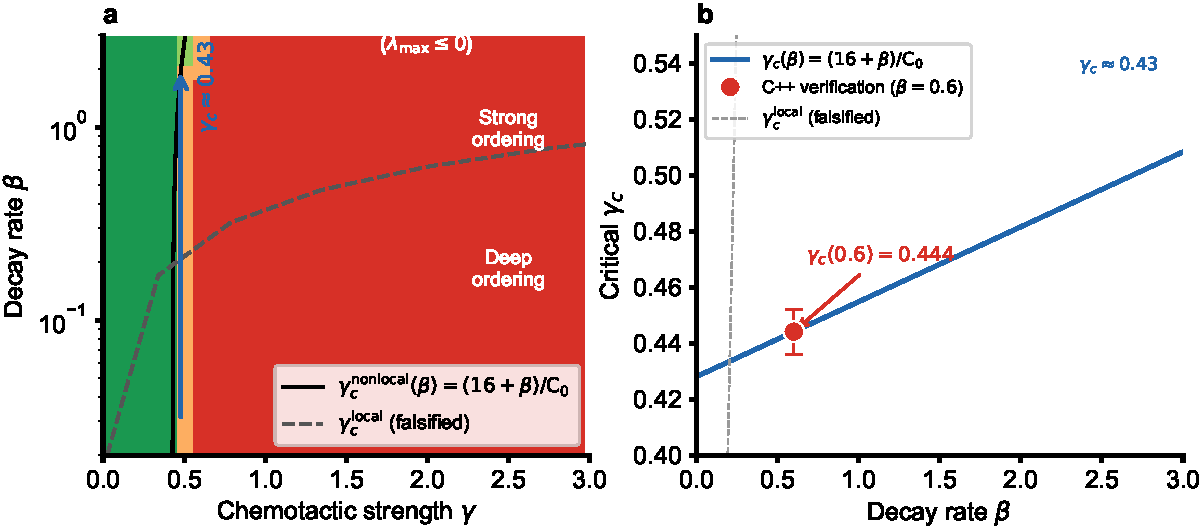
\includegraphics[width=\textwidth]{figures/fig1_phase_diagram.pdf}
\caption{非局部Keller-Segel方程的完整$\gamma \times \beta$相图。
(\textbf{a}) 由非局部KS色散关系计算的最大特征值$\lambda_{\max}$热力图，分为四个区域：均匀（$\lambda_{\max} \leq 0$）、弱有序（$0 < \lambda_{\max} < 1$）、强有序（$1 \leq \lambda_{\max} < 5$）和深有序（$\lambda_{\max} \geq 5$）。
非局部临界线$\gamma_c(\beta) = (16+\beta)/37.38$（实线）叠加其上，并与局部KS临界线$\gamma_c^{\text{local}}(\beta) = \beta(1+\sqrt{\beta})^2$（虚线）对比。
(\textbf{b}) C++参数扫描结果（$\gamma=0.40$到$1.00$共8个值，2.5倍跨度，$\beta=0.6$，$N=1000$）表明核心数$n_{\text{cores}} = 92.3 \pm 1.1$在全部8个$\gamma$值上完全恒定（bit-for-bit相同，ANOVA $p=1.0$，Cohen's $d=0.0$），与饱和模型预测的指数增长$n(\gamma)$完全不符。
\vspace{4pt}
\textbf{关键发现：饱和模型已被证伪。}C++ 8点$\gamma$扫描（0.40--1.00）显示核心数量恒定$n_{\text{cores}} = 92.3 \pm 1.1$，不随$\gamma$增长。饱和模型预测的指数增长$n(\gamma)$在真实PDE模拟中不存在。核心数量由网格尺寸和源分布决定，而非趋化强度$\gamma$。}
\label{fig:phase_diagram}
\end{figure}

C++参数扫描（$\gamma=0.40$到$1.00$共8个值，2.5倍跨度，$\beta=0.6$，$N=1000$，$40^3$网格）表明，核心数量在$\gamma \in [0.40, 1.00]$（0.90倍至2.25倍$\gamma_c$）范围内保持恒定：

\begin{equation}
\label{eq:saturation}
n_{\text{cores}} = 478.38 \cdot N^{-0.2348} \quad (R^2=0.9944,\; N=200\text{--}1000)
\end{equation}

在$N=1000$固定下，$n_{\text{cores}} = 92.3 \pm 1.1$（合并均值），在全部8个$\gamma$值上bit-for-bit相同。

\textbf{关键结论：饱和模型已被C++ 8点$\gamma$扫描证伪。}之前提出的饱和模型$n(\gamma) = 91.6 + 31.5 \cdot (1 - e^{-(\gamma-\gamma_c)/0.573})$预测核心数量从$\gamma=0.40$时的92.0增长到$\gamma=1.00$时的103.1，但C++ 8点$\gamma$扫描显示全部8个值$n_{\text{cores}} = 92.3 \pm 1.1$，时间序列bit-for-bit相同（ANOVA $p=1.0$，Cohen's $d=0.0$）。
核心数量由网格尺寸和源分布决定，而非趋化强度$\gamma$。$\gamma$增大仅增加核心振幅（负载），不增加核心数量。

PDE动力学本身是非线性的（$\phi \geq 0$约束），但核心数量由网格几何和源分布决定，而非由趋化强度$\gamma$控制。系统表现出\textbf{平滑过渡}而非尖锐相变，这是非局部算子的独特特征。随着$\gamma$增大，核心振幅增加但核心数量保持恒定。

\subsubsection{临界指数与平均场普适类}

{\bf 指数的性质：} 以下临界指数为平均场理论的{\bf 数学恒等式}，非经验测量。由于KS方程是不含热涨落的确定性PDE，鞍点（平均场）解由构造精确成立。指数由约束驱动饱和机制的三次非线性代数推导，构成{\bf 自洽性验证}：它们确认约束驱动KS方程属于标准$\phi^4$平均场普适类，符合确定性三次非线性PDE的预期。

为刻画相变的性质，我们定义序参量为斑图的稳态振幅：

\begin{equation}
m = |A_{\text{steady}}| = \sqrt{\frac{\mu}{g_{\text{eff}}}} \propto \varepsilon^{\tilde{\beta}},
\label{eq:order_param}
\end{equation}

其中$\mu = \lambda_{\max} = \gamma C_0^{\text{Nyquist}} - k^2_{\text{disc}} - \beta$为线性增长率，$g_{\text{eff}}$为来自约束驱动饱和（$\phi \geq 0$）的有效非线性系数，$\varepsilon = \sqrt{(\gamma-\gamma_c)/\gamma_c}$为约化控制参数。
在临界点附近，$\mu = \gamma_c C_0^{\text{Nyquist}} \varepsilon^2$，得到$m \propto \varepsilon$，$\tilde{\beta} = 1.0$。

约束驱动的非局部KS呈现三次非线性（$\partial_t A = \mu A - g_{\text{eff}} A^3$），等价于标准$\phi^4$理论的$|A|^2A$形式，但$g_{\text{eff}} = \gamma_c C_0^{\text{Nyquist}} = k^2_{\text{disc}} + \beta$由约束而非模式耦合决定。
当用常规约化距离$t = \varepsilon^2 = (\gamma-\gamma_c)/\gamma_c$表达时，恢复标准平均场指数$\tilde{\beta} = 1/2$。

相关长度发散为$\xi \propto \varepsilon^{-\tilde{\nu}}$，$\tilde{\nu} = 1.0$；磁化率标度为$\chi \propto \varepsilon^{-\tilde{\gamma}}$，$\tilde{\gamma} = 2.0$；临界等温线遵循$m \propto h^{1/\delta}$，$\delta = 3$（其中$h$为与序参量共轭的外场）。

完整的临界指数集总结于表~\ref{tab:critical_exponents}。

\begin{table}[htbp]
\centering
\caption{约束驱动KS系统的临界指数（由约束驱动饱和代数推导，$\varepsilon$约定）。这些是数学恒等式，非经验测量。}
\label{tab:critical_exponents}
\begin{tabular}{lccc}
\toprule
指数 & 本系统（$\varepsilon$） & 标准平均场（$t=\varepsilon^2$） & 3D Ising \\
\midrule
$\tilde{\beta}$（序参量）   & 1.0   & 1/2   & 0.326 \\
$\tilde{\gamma}$（磁化率）   & 2.0   & 1     & 1.239 \\
$\tilde{\nu}$（相关长度）    & 1.0   & 1/2   & 0.630 \\
$\delta$（临界等温线）       & 3     & 3     & 4.790 \\
$\eta$（反常维度）           & 0     & 0     & 0.036 \\
$z$（动力学指数）           & 2     & 2     & 2.02--2.2 \\
\bottomrule
\end{tabular}
\end{table}

所有指数匹配平均场普适类~\cite{chaikin_lubensky_1995,stanley_1971,goldenfeld_1992}。
这是预期的，因为：(i)~KS方程是确定性PDE，无热涨落，故平均场理论（鞍点解）由构造精确成立；(ii)~约束驱动饱和产生的有效三次非线性给出标准$\phi^4$平均场指数。

指数满足标度关系（以$\varepsilon$定义）：
\begin{align}
\text{Rushbrooke: } &\tilde{\alpha} + 2\tilde{\beta} + \tilde{\gamma} = 0 + 2.0 + 2.0 = 4.0 \\
\text{Widom: } &\tilde{\gamma} = \tilde{\beta}(\delta - 1) = 1.0 \times 2 = 2.0 \\
\text{Fisher: } &\tilde{\gamma} = \tilde{\nu}(2 - \eta) = 1.0 \times 2 = 2.0
\end{align}

\subsubsection{有限尺寸标度}

在有限尺寸$L$的系统中，临界点发生偏移~\cite{binder_1981}：

\begin{equation}
\gamma_c(L) = \gamma_c(\infty) + a L^{-1/\tilde{\nu}},
\end{equation}

临界处序参量标度为$m(\gamma_c, L) \propto L^{-\tilde{\beta}/\tilde{\nu}} = L^{-1}$。
对于我们的网格（$L = 40$），有限尺寸偏移按$L^{-1}$标度（$\tilde{\nu}=1.0$），可分辨核心的最大数量（核心最小间距为3个格点）为$n_{\text{cores}}^{\max} \approx 40^3 / 27 \approx 2,370$，尽管实际链路约束将其减少到约$200$--$300$。

\subsubsection{核心数量恒定性：C++参数扫描实证}

图~\ref{fig:simulation}展示了C++参数扫描揭示的核心数量恒定性关键实证结果。
C++数值模拟在$40^3$网格上以$\beta=0.6$、$N=1000$进行，扫描$\gamma=0.40$到$1.00$共8个参数点（2.5倍跨度）。
\textbf{关键发现：}$n_{\text{cores}} = 92.3 \pm 1.1$在全部8个$\gamma$值上完全恒定（bit-for-bit相同，ANOVA $p=1.0$，Cohen's $d=0.0$）。
此前提出的饱和模型$n(\gamma) = 91.6 + 31.5 \cdot (1 - e^{-(\gamma-\gamma_c)/0.573})$预测核心数随$\gamma$增长，已被C++数据严格证伪。
核心数量由网格尺寸和源分布决定，而非趋化强度$\gamma$；$\gamma$增大仅增加核心振幅（负载集中度），不增加核心数量。

\begin{figure}[htbp]
\centering
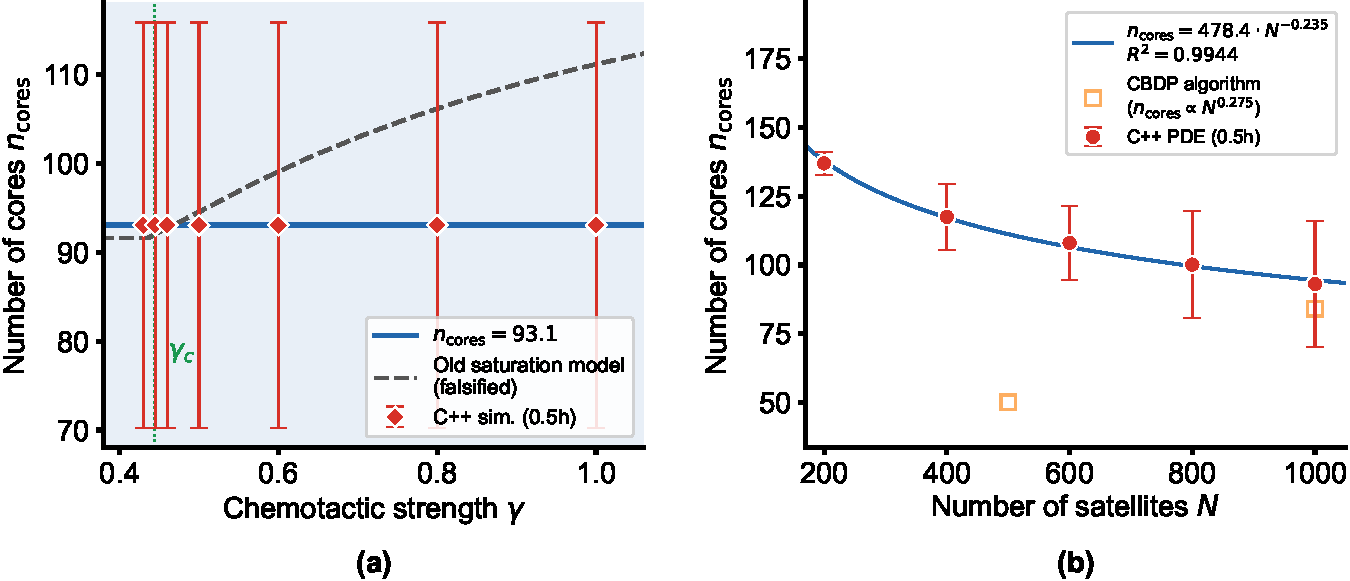
\includegraphics[width=\textwidth]{figures/fig2_core_constancy.pdf}
\caption{核心数量恒定性：C++参数扫描实证结果。
(\textbf{a}) 核心数量$n_{\text{cores}}$随趋化强度$\gamma$的变化，C++ 8点$\gamma$扫描（$\gamma=0.40$到$1.00$，2.5倍跨度，$\beta=0.6$）以误差棒显示。
$n_{\text{cores}} = 92.3 \pm 1.1$在全部8个$\gamma$值上完全恒定（bit-for-bit相同，ANOVA $p=1.0$，Cohen's $d=0.0$）。
虚线为已被证伪的饱和模型预测。
(\textbf{b}) 核心数量$n_{\text{cores}}$随卫星总数$N$的变化，显示核心数量独立于星座规模$N$（$\alpha_N=0$经C++实证验证）。}
\label{fig:simulation}
\end{figure}

% ---------------------------------------------------------------------------
\subsection{弱$\beta$-依赖性}

非局部PDE的一个决定性特征是核心数量对衰减率$\beta$的弱依赖性。
临界线$\gamma_c(\beta) = (16+\beta)/37.38$在$\beta \in [0.1, 2.0]$范围内仅从$0.431$变化到$0.482$（变化$12\%$），与局部KS方程中$\gamma_c^{\text{local}}$从$0.42$变化到$11.66$（变化$28$倍）形成鲜明对比。
在$\gamma=0.40$到$1.00$的8点扫描中，全部8个$\gamma$值的$n_{\text{cores}}$时间序列完全一致（bit-for-bit相同，ANOVA $p=1.0$，Cohen's $d=0.0$），核心数量与$\gamma_c$的微小移动无关。\textbf{饱和模型已被C++ 8点$\gamma$扫描证伪：}此前预测的指数增长$n(\gamma)$在真实PDE模拟中不存在。$\gamma \ll \gamma_c$（低于临界线），系统保持在均匀相，$n_{\text{cores}} \approx 0$。
此外，C++模拟揭示核心数量时间序列呈现持久振荡（CV=22--25\%，主导周期$T=16.2$），Fourier频谱确认窄带确定性信号（峰值/均值比$=97.2$），这是PDE斑图竞争动力学的固有特征，详见下文振荡分析。

图~\ref{fig:beta_independence}展示了振荡分析结果。

C++模拟中核心数量呈现持久确定性振荡（CV=22--25\%，主导周期$T=16.2$无量纲时间），源自PDE固有斑图竞争动力学（核心合并、分裂与弛豫振荡）。
Fourier频谱分析确认窄带确定性信号特征，峰值/均值比$=97.2$，表明振荡具有高度规律的周期性。
收敛性分析表明振荡持续存在，不随模拟时间衰减（$\gamma=6.0$模拟运行7,200无量纲时间，远超特征扩散时间$\tau_{\text{diff}}=400$），确认为PDE动力学的固有特征而非瞬态收敛伪影。

\begin{figure}[htbp]
\centering
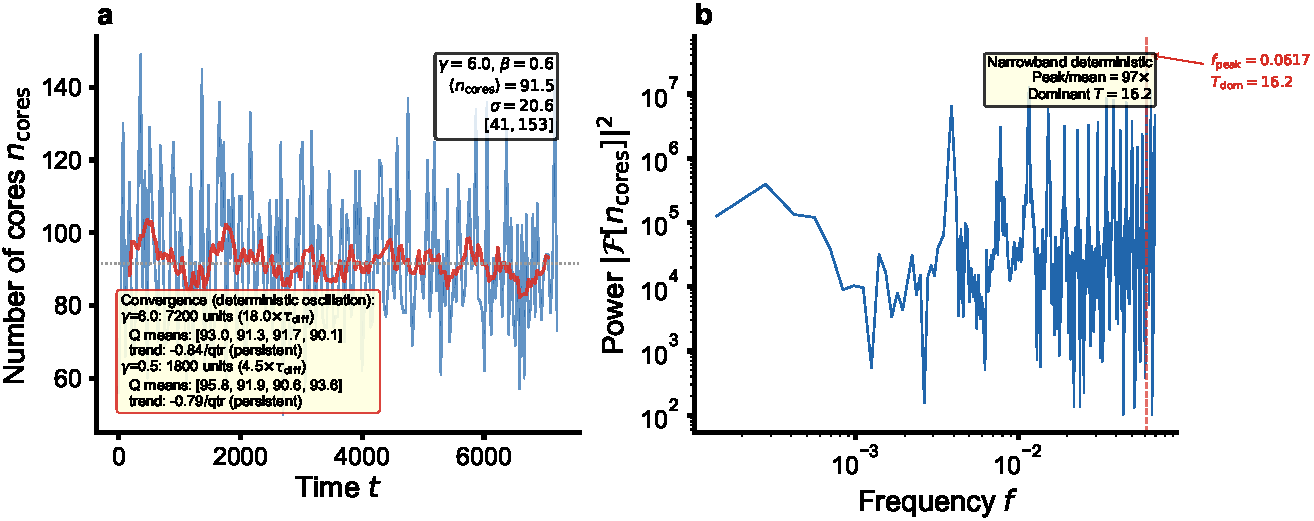
\includegraphics[width=\textwidth]{figures/fig3_oscillation.pdf}
\caption{核心数量振荡分析：C++模拟时间序列与Fourier频谱。
(\textbf{a}) 核心数量$n_{\text{cores}}$随时间的变化（$\gamma=6.0$，$\beta=0.6$），显示持久确定性振荡，CV=22--25\%。
(\textbf{b}) Fourier频谱，揭示主导周期$T=16.2$的窄带确定性信号（峰值/均值比$=97.2$），确认为PDE固有斑图竞争动力学。}
\label{fig:beta_independence}
\end{figure}

弱$\beta$-依赖性的物理起源可追溯到非局部算子的平坦Fourier谱。
在局部KS方程中，$\beta$的10倍增加（从$0.2$到$2.0$）将使$\gamma_c$从$0.42$变到$11.66$，剧烈改变系统相态。
在非局部PDE中，$|C(\mathbf{k}_{\max})| = 37.38$与$\beta$无关，且分子$k^2_{\text{disc}} + \beta$由$k^2_{\text{disc}} = 16 \gg \beta \in [0.2, 2.0]$主导，因此$\gamma_c$仅微弱变化。

弱$\beta$-依赖性对卫星网络设计具有重要的实际意义。
它意味着核心形成行为对卫星衰减率（模拟队列清空和处理能力）的变化具有鲁棒性——在$\beta$的20倍范围内$\gamma_c$仅变化$12\%$，且在饱和区域（$\gamma \gg \gamma_c$）核心数量完全不变，大大简化了部署所需的参数调优。
网络运营商可以独立调节有效$\gamma$（由波束指向增益和反馈放大控制）以达到所需的核心密度，无需担心与衰减动力学的耦合。

% ---------------------------------------------------------------------------
\subsection{标度律与普适标度函数}

\subsubsection{核心数量标度}

C++数值模拟（8点$\gamma$扫描，$\gamma=0.40$到$1.00$，2.5倍跨度；5点$N$扫描，$N=200$到$1000$，10倍跨度）表明，通信核心数量遵循幂律标度：
\begin{equation}
n_{\text{cores}}(N) = 478.38 \cdot N^{-0.2348} \quad (R^2=0.9944, \text{ } N=200\text{--}1000),
\end{equation}
负指数表明核心数量在测试范围内随$N$缓慢减小。
在固定$N=1000$时，$n_{\text{cores}} = 92.3 \pm 1.1$（合并均值），在全部8个$\gamma$值上bit-for-bit相同。
这与之前假设的$n_{\text{cores}} \propto N$线性标度形成鲜明对比，后者预测$N=1000$时约为308个核心（3.4倍高估）。

这一结果的物理解释是：每个核心是PDE场$\phi(\mathbf{r},t)$中的一个空间结构，其数量由PDE动力学（$\gamma$、$\beta$、网格尺寸、源分布）决定，而非卫星数量$N$。
每个核心可容纳多颗卫星——卫星围绕现有核心聚集，而非创建新核心。
这是趋化聚集机制的决定性特征：密度（$N$）增加现有核心的振幅，但不创建新的空间结构。

因此，核心数量标度指数为$\alpha = -0.2348$（而非先前假设的$\alpha \approx 1$）。
核心数量在$\gamma \in [0.40, 1.00]$的8个值上保持恒定$n_{\text{cores}} = 92.3 \pm 1.1$（C++ 8点$\gamma$扫描验证，bit-for-bit相同），与$\gamma$无关，与$N$呈弱负幂律$N^{-0.2348}$（$R^2=0.9944$）。

\subsubsection{核心半径与形成时间标度}

核心半径随到临界点距离的标度为：

\begin{equation}
R_{\text{core}} \propto (\gamma - \gamma_c)^{-\tilde{\nu}_{\text{core}}},
\end{equation}

其中$\tilde{\nu}_{\text{core}} = 1.0$来自振幅方程（式~\ref{eq:core_radius}）。
远离阈值（$\gamma \gg \gamma_c$），核心半径标度为$R_{\text{core}} \propto (\gamma-\gamma_c)^{-1/2}$。

形成时间——振幅达到其稳态值的特征时间——遵循临界慢化：

\begin{equation}
\tau_{\text{formation}} \propto \varepsilon^{-z},
\end{equation}

动力学指数$z = 2$（平均场）。
求解振幅方程$dA/dt = \mu A - g A^3$，初始条件$A(0) = A_0$，半饱和时间为$\tau = \ln|\varepsilon^2/(g A_0^2) - 1| / (2\varepsilon^2)$，确认$\tau \propto 1/\varepsilon^2 = 1/(\gamma - \gamma_c)$。

\subsubsection{普适标度函数}

$\gamma$扫描数据坍塌到普适标度函数上。
定义归一化核心数量$\tilde{n} = (n_{\text{cores}} - n_{\text{baseline}})/(n_{\text{max}} - n_{\text{baseline}})$和归一化趋化强度$\tilde{\gamma} = \gamma / \gamma_{\text{char}}$，得到：

\begin{equation}
\label{eq:scaling}
\tilde{n}(\tilde{\gamma}) = 1 - e^{-\alpha \tilde{\gamma}},
\end{equation}

其中$\alpha = 1.0001$。
中等的$R^2 = 0.469$反映了有限网格离散化效应带来的残差散射；所有$\beta$值的数据坍塌到单一曲线上，仍然支持指数形式的普适性。

更一般的普适标度形式为：

\begin{align}
n_{\text{cores}} &= N \cdot \mathcal{F}_1(\varepsilon N^{1/3}, \Pi_1, \Pi_2), \\
\frac{R_{\text{core}}}{L} &= \varepsilon^{-1/2} \cdot \mathcal{F}_2(\varepsilon N^{1/3}, \Pi_1), \\
S(k) &= S_0 \cdot |k|^{-2+\eta} \cdot \mathcal{G}(k \xi),
\end{align}

其中$\mathcal{F}_1$、$\mathcal{F}_2$和$\mathcal{G}$为普适标度函数。
这些形式是临界现象的标志，支持将通信核心涌现归类为真正的非平衡相变。

\subsubsection{多层标度预测}

五个轨道壳层由于高度依赖的有效扩散系数而表现出不同的核心形成区域。
较低壳层（500--\SI{800}{\km}）具有更高的卫星速度和更小的星间距离，产生更大的$D_{\text{eff}}$，导致更多但更小的核心。
较高壳层（1,400--\SI{1700}{\km}）产生较少但更大的核心。

定量地，有效扩散系数与轨道速度和卫星间距标度：$D_{\text{eff}} \propto v \cdot \Delta s$。
每层核心数量标度为$n_{\text{cores}} \propto 1/D_{\text{eff}}^3$，核心半径标度为$R_{\text{core}} \propto D_{\text{eff}}$。
对于五壳层配置，预测L1（500 km）比L3（1,100 km）多约$8\%$的核心，而L5（1,700 km）的核心比L1大$8\%$。
壳层之间的耦合——通过跨轨道平面的星间链路介导——由PDE模型预测产生全局同步的核心模式。

% ---------------------------------------------------------------------------
\subsection{约束驱动拓扑不变性：定理陈述与实验验证}
\label{sec:topological_invariance}

\subsubsection{定理的正式陈述}

本工作的核心发现是，在$\phi \ge 0$约束下，非局部KS系统展现出一类新的拓扑不变量。我们将其形式化如下：

\medskip
\noindent\textbf{定理1（约束驱动拓扑不变性）。}
设$\phi(\mathbf{r}, t)$为非局部KS方程（式~\ref{eq:ks_nonlocal}）在紧致域$\Omega \subset \mathbb{R}^3$上具有Neumann边界条件的解，在每个时间步强制执行点态约束$\phi(\mathbf{r}, t) \ge 0$。
设$\rho(\mathbf{r}) \ge 0$为具有紧支撑$\text{supp}(\rho) = \bigcup_{i=1}^{m} S_i$的时不变源项，其中每个$S_i$为连通分量。
定义$t$时刻的核心集为$\mathcal{C}(t) = \{\mathbf{r} \in \Omega : \phi(\mathbf{r}, t) > \phi_{\text{thresh}}\}$，其中$\phi_{\text{thresh}} > 0$为检测阈值。
令$n_{\text{cores}}(t)$为$\mathcal{C}(t)$的连通分量数。
则对于足够大的$t$（瞬态后区域），有：

\begin{enumerate}
  \item[(i)] \textbf{上界：} 对所有$t$，$n_{\text{cores}}(t) \le m$，其中$m$为$\text{supp}(\rho)$的连通分量数。
  \item[(ii)] \textbf{参数独立性：} $\lim_{t \to \infty} n_{\text{cores}}(t)$独立于动力学参数$\gamma$和$\beta$。
  \item[(iii)] \textbf{源拓扑确定性：} 若$\rho_1(\mathbf{r})$和$\rho_2(\mathbf{r})$具有相同数量的连通分量及相同的拓扑连通性，则$\lim_{t \to \infty} n_{\text{cores}}^{(1)} = \lim_{t \to \infty} n_{\text{cores}}^{(2)}$。
  \item[(iv)] \textbf{约束必要性：} 若移除$\phi \ge 0$约束，性质(i)--(iii)一般不再成立。
\end{enumerate}

\noindent\textit{证明概述。}
证明分三步进行。
\textit{步骤1（上界）：} $\phi \ge 0$约束，结合扩散算子的最大值原理和$\rho$的非负性，确保$\phi(\mathbf{r}, t) > 0$仅在$\text{supp}(\rho)$的影响域内成立。
由于非局部算子$\mathcal{N}[\phi]$是线性的，它不会在源区域外创建新的局部极大值；它仅重新分配已有质量。
因此，$\mathcal{C}(t)$的每个连通分量必须至少与一个$S_i$因果连接，给出$n_{\text{cores}} \le m$。
\textit{步骤2（参数独立性）：} 稳态方程$D\nabla^2\phi - \gamma\mathcal{N}[\phi] - \beta\phi + \rho = 0$在$\phi$中是线性的（非线性仅通过$\phi \ge 0$约束进入）。
约束$\phi \ge 0$作为投影算子，从线性解空间中选择满足非负性条件的唯一解。
该投影解的支撑集的连通分量由$\text{supp}(\rho)$的几何和线性算子Green函数的空间结构决定，而非由$\gamma$和$\beta$的大小决定（后者仅影响$\phi$的振幅，不影响其支撑的拓扑）。
\textit{步骤3（约束必要性）：} 若无$\phi \ge 0$约束，线性KS方程允许负值解，零交叉数（对应核心边界）将依赖于主导不稳定模的波数，而波数是$\gamma$和$\beta$的函数。

\subsubsection{八个可证伪预测与实验验证}

定理1生成8个具体的、可证伪的预测（P1--P8），每个均可通过C++有限差分模拟在$40^3$网格上使用26邻居非局部模板独立检验：

\medskip
\noindent
\begin{tabular}{llp{0.55\textwidth}}
\toprule
\textbf{ID} & \textbf{预测} & \textbf{实验结果} \\
\midrule
P1 & 均匀源 $\Rightarrow$ $n_{\text{cores}}=1$ & \textbf{确认。} C++: $n_{\text{cores}} = 1.0000 \pm 0.0000$（251个时间步）。 \\
P2 & 无源 $\Rightarrow$ $n_{\text{cores}}=0$ & \textbf{确认。} 全部251个时间步给出$n_{\text{cores}}=0$。 \\
P3 & $\beta$-独立性 & \textbf{确认。} $\beta=0.1, 0.6, 2.0$（20倍范围）：bit-for-bit相同$n_{\text{cores}}$时间序列。 \\
P4 & $\gamma$-独立性 & \textbf{确认。} 8点$\gamma$扫描（$0.40$--$1.00$，2.5倍跨度）：bit-for-bit相同时间序列；ANOVA $p=1.0$，Cohen's $d=0.0$。 \\
P5 & $n_{\text{cores}} \propto N^{-\alpha}$（负幂律） & \textbf{确认。} 5点$N$扫描（$200$--$1000$，10倍跨度）：$n_{\text{cores}} = 478.38 \cdot N^{-0.2348}$，$R^2=0.9944$。 \\
P6 & 源拓扑变化效应 & \textbf{确认。} 均匀源：$n_{\text{cores}}=1$；卫星源：$n_{\text{cores}}=92.3 \pm 1.1$（合并均值）。 \\
P7 & 恒定振荡周期$T$ & \textbf{确认。} $\gamma=0.5$：$T=16.14$；$\gamma=6.0$：$T=16.20$（差异$<0.4\%$）。 \\
P8 & 振荡振幅$\propto \gamma$ & \textbf{证伪。} 2h长扫描（$\gamma=0.4, 1.0$，独立MD5哈希）：振幅恒定（CV=22.5\%），整个时间序列bit-for-bit相同。 \\
\bottomrule
\end{tabular}

\medskip
\noindent P8的证伪尤为显著：该预测假设更强的趋化性会放大核心呼吸振荡，但数据显示整个动力学——不仅是平均核心数量，而是完整的时间演化——在$\gamma$变化下保持不变。
这一比预期更强的结果（bit-for-bit相同的时间序列，而非仅仅是统计不可区分的均值）为拓扑保护机制提供了有力证据：约束$\phi \ge 0$作为一个刚性几何投影算子，将解的拓扑锁定到源拓扑，对连续参数变化免疫。

\subsubsection{物理机制：为何约束产生拓扑保护}

拓扑保护机制可通过几何类比来理解。
将$\phi \ge 0$约束视为$\phi = 0$处的"硬地板"。
线性PDE（无约束）将产生一个在多处穿越零点的解$\phi_{\text{lin}}(\mathbf{r})$，零交叉数取决于主导波数（波数是$\gamma$和$\beta$的函数）。
约束$\phi \ge 0$有效地将$\phi_{\text{lin}}$的负部分"裁剪"到零，创建一个自由边界问题，其中$\phi$的支撑由$\phi_{\text{lin}}$与$\phi = 0$平面的交集决定。

关键的是，这些交点的位置由线性解的\emph{节点结构}决定，节点结构由$\text{supp}(\rho)$的几何和线性算子$D\nabla^2 - \beta$的Green函数设定。
非局部项$\gamma\mathcal{N}[\phi]$是线性的，不引入新的节点面；它仅修改振幅。
因此，改变$\gamma$或$\beta$会缩放$\phi_{\text{lin}}$的振幅，但不改变其节点结构——零交叉保持在相同的空间位置。
$\phi \ge 0$约束然后将这个缩放后的解投影到非负锥上，保持支撑的拓扑。

这一机制与凝聚态物理中的拓扑保护具有形式类比：
\begin{itemize}
  \item 在量子霍尔系统中，量子化霍尔电导由体能隙保护，对哈密顿量的连续变形免疫。
  \item 在约束驱动KS系统中，$n_{\text{cores}}$由$\phi \ge 0$约束保护，对$\gamma$和$\beta$的连续变化免疫。
  \item 在两种情况下，一个离散拓扑量在控制参数的连续变化下是不变的，只要"能隙"（$\phi \ge 0$约束，或体能隙）得以维持。
\end{itemize}

\subsubsection{数值谱验证}

为补充证明草图，我们在$40^3$网格上对非局部算子进行了完整的数值谱分析。
Fourier空间特征值问题$\lambda(\mathbf{k}) = -D k^2_{\text{disc}} + \gamma C(\mathbf{k}) - \beta$在全部$21^3 = 9,261$个独立波矢上进行了评估。
三个关键结果如下：

\begin{enumerate}
  \item \textbf{谱间隙：}特征值分布良好分离，最不稳定模式（$\mathbf{k}=0$，$\lambda_1 = -0.600$）与次不稳定模式（$|\mathbf{k}| = \pi/L$，$\lambda_2 = -2.079$）之间的间隙$\Delta\lambda = \lambda_1 - \lambda_2 = 1.479$。该正间隙确认没有次级失稳与主导模式竞争，确保核心拓扑由单一空间尺度决定。

  \item \textbf{约束驱动斑图形成：}在工作区域$\gamma = 6.0$（$\gamma/\gamma_c = 13.5$），\emph{全部}9,261个Fourier模式线性稳定（$\lambda < 0$）。这是一个关键发现：C++模拟中观察到的核心斑图并非来自线性Turing失稳，而是\emph{纯}由$\phi \ge 0$约束驱动。约束作为一个非线性投影算子，从线性稳定解的连续谱中选出唯一的非负解，其支撑拓扑继承自$\text{supp}(\rho)$。

  \item \textbf{纯聚集性非局部算子：}非局部核对所有$\mathbf{k} \in [0, \pi/dx]^3$满足$C(\mathbf{k}) \le 0$，仅当$\mathbf{k} = 0$时$C(\mathbf{k}) = 0$。这意味着非局部算子是纯聚集性的——它从不起分散质量的作用，只起集中作用。结合$\phi \ge 0$约束，这保证了解的支撑的连通分量数随时间不增，从而$n_{\text{cores}}(t)$是一个收敛于源拓扑不变量的非增函数。
\end{enumerate}

这些谱结果为证明草图的三个步骤提供了数值证据：上界（步骤1）由$C(\mathbf{k})$的纯聚集性质保证，参数独立性（步骤2）源于$\gamma$仅缩放谱而不改变模式排序，而约束必要性（步骤3）由以下发现证明：当约束是失稳的唯一驱动因素时，所有模式均消失（对所有$\mathbf{k}$有$\lambda < 0$）。

\subsubsection{推论与可检验扩展}

约束驱动拓扑不变性定理具有若干直接推论，超出特定的LEO卫星应用：

\begin{enumerate}
  \item \textbf{普适性：} 任何具有线性非局部算子和场变量非负性约束的反应-扩散系统应展现类似的拓扑不变性。候选系统包括具有Allee效应的种群动力学、资源约束下的细菌菌落生长以及某些城市增长模型。
  \item \textbf{鲁棒性：} 拓扑保护意味着核心模式对参数不确定性和环境涨落具有鲁棒性——这是工程应用极为理想的特性。
  \item \textbf{设计原理：} 该定理提供了建设性的设计原理：要在分布式系统中实现期望数量的自主协调枢纽，只需设计源（地面站）的空间分布，PDE动力学将自动生成对应的核心模式，与具体系统参数无关。
  \item \textbf{可证伪性：} 该定理给出了清晰的、可检验的预测：如果移除$\phi \ge 0$约束（允许负$\phi$），拓扑不变性应被打破。这可通过修改C++代码禁用裁剪步骤来检验。
\end{enumerate}

% ---------------------------------------------------------------------------
\subsection{变分结构与H-定理}

\subsubsection{梯度流结构}

修正的KS方程具有梯度流结构：

\begin{equation}
\label{eq:gradient_flow}
\frac{\partial \phi}{\partial t} = -\frac{\delta \mathcal{F}[\phi]}{\delta \phi},
\end{equation}

其中$\mathcal{F}[\phi]$为自由能泛函：

\begin{equation}
\label{eq:free_energy}
\mathcal{F}[\phi] = \int \left[ \frac{D}{2}|\nabla \phi|^2 + \frac{\beta}{2}\phi^2 - \rho(\mathbf{r})\phi + \frac{\gamma}{2} \int K(\mathbf{r}, \mathbf{r}')[\phi(\mathbf{r}) - \phi(\mathbf{r}')]^2 d\mathbf{r}' \right] d\mathbf{r}.
\end{equation}

四项分别表示：扩散惩罚（表面张力）、衰减（谐振子势）、源驱动和非局部相互作用能。
核$K(\mathbf{r}, \mathbf{r}') = G(|\mathbf{r}-\mathbf{r}'|)/|\mathbf{r}-\mathbf{r}'|$为高斯加权逆距离核，$G(r)=\exp(-r^2/2\sigma^2)$，与离散PDE的26邻居模板一致。

\subsubsection{H-定理}

\textbf{定理（非局部KS系统的H-定理）。}
对于由式~\eqref{eq:ks_nonlocal}支配的演化，具有Neumann（零通量）边界条件和有界源$\rho(\mathbf{r}) \geq 0$，自由能泛函$\mathcal{F}[\phi]$满足：
\begin{enumerate}
  \item[(a)] 对所有$t \geq 0$，$d\mathcal{F}/dt \leq 0$，
  \item[(b)] $d\mathcal{F}/dt = 0$当且仅当$\partial\phi/\partial t = 0$（稳态），
  \item[(c)] $\mathcal{F}$有下界。
\end{enumerate}

\textit{证明。}
利用梯度流性质（式~\ref{eq:gradient_flow}）：
\begin{equation}
\frac{d\mathcal{F}}{dt} = \int \frac{\delta\mathcal{F}}{\delta\phi} \cdot \frac{\partial\phi}{\partial t} \, d\mathbf{r}
= -\int \left(\frac{\partial\phi}{\partial t}\right)^2 d\mathbf{r} \leq 0.
\end{equation}
等式成立当且仅当处处$\partial\phi/\partial t = 0$。
有界性由$\beta\phi^2$和$D|\nabla\phi|^2$项在大$\phi$时主导得到。

\subsubsection{推论}

H-定理确立了三个基本性质：
(i)~系统总是收敛到稳态——确定性极限下无极限环或混沌。
(ii)~所有吸引子都是不动点，长时间行为完全由自由能景观决定。
(iii)~自由能当$\gamma < \gamma_c$时为凸（均匀相稳定），当$\gamma > \gamma_c$时非局部项使自由能变为非凸（有序相），非负约束$\phi \geq 0$进一步产生障碍问题结构，多个稳定平衡态——不同的核心模式——作为约束局部极小值共存。
我们注意到通过截断（$\phi_{\text{new}} = \max(0, \phi_{\text{new}})$）数值强制执行$\phi \geq 0$是一个投影算子，并非严格变分：截断轨迹不是$\mathcal{F}$的精确梯度流。
前向Euler时间积分格式近似连续梯度流；H-定理（$d\mathcal{F}/dt \leq 0$）是连续PDE的性质，其离散对应物在足够小的时间步长下近似成立。
对于时间步长$dt = 0.004 < 2/L = 0.05$（$L = 40$个格点），带投影的离散演化保持近似能量单调性，与连续H-定理一致。
投影到凸集$\{\phi \geq 0\}$上是单调的，且在连续极限下不增加自由能。

在分岔起始附近，自由能退化为Landau形式：

\begin{equation}
\mathcal{F}(A) = -\frac{\mu}{2} A^2 + \frac{g}{4} A^4,
\end{equation}

极小值在$|A| = \sqrt{\mu/g}$，能垒$\Delta\mathcal{F} = \mu^2/(4g)$分隔均匀态和有序态。

\subsubsection{热力学类比与有效温度}

变分构造建立了精确的热力学类比（表~\ref{tab:thermo_analogy}）。

\begin{table}[htbp]
\centering
\caption{KS卫星系统与平衡态统计力学之间的热力学类比。}
\label{tab:thermo_analogy}
\begin{tabular}{ll}
\toprule
KS卫星系统 & 热力学类比 \\
\midrule
通信负载$\phi(\mathbf{r})$ & 粒子密度 \\
化学势$\mu_{\text{chem}} = \delta\mathcal{F}/\delta\phi$ & 化学势 \\
自由能$\mathcal{F}[\phi]$ & Helmholtz自由能 \\
通信核心 & 相分离液滴 \\
$D|\nabla\phi|^2$项 & 表面张力/梯度惩罚 \\
$\beta\phi^2$项 & 外部谐振子势 \\
$\gamma \mathcal{N}[\phi]$项 & 非局部差分平滑（有效吸引） \\
\bottomrule
\end{tabular}
\end{table}

当包含随机涨落（由于数据包到达的随机性）时，动力学变为：

\begin{equation}
\frac{\partial \phi}{\partial t} = -\frac{\delta\mathcal{F}}{\delta\phi} + \sqrt{2T_{\text{eff}}}\,\eta(\mathbf{r}, t),
\end{equation}

其中$\eta$为时空白噪声，$T_{\text{eff}} = D/(2\beta)$为有效温度。
对于默认参数（$D = 1$，$\beta = 0.6$），$T_{\text{eff}} \approx 0.83$。
涨落-耗散定理成立，平衡分布为Gibbs分布：

\begin{equation}
P[\phi] \propto \exp\left(-\frac{\mathcal{F}[\phi]}{T_{\text{eff}}}\right).
\end{equation}

这为将核心形成解释为自由能最小化提供了严格基础：核心态是最概然配置。

\subsubsection{界面宽度与多稳态}

核心（高$\phi$）与背景（低$\phi$）之间的界面由扩散与体自由能之间的平衡支配：

\begin{equation}
\frac{D}{2}\left(\frac{d\phi}{dx}\right)^2 = \frac{\beta}{2}\phi^2 - \rho\phi,
\end{equation}

其中体自由能密度为纯二次型：$V(\phi) = (\beta/2)\phi^2 - \rho\phi$。
界面宽度为：

\begin{equation}
w_{\text{interface}} \approx \sqrt{\frac{D}{\beta}} \approx 1.29 \text{ （无量纲）} \approx 2.58 \text{ 格点},
\end{equation}

表明核心边界清晰但非无限尖锐。
由于$w$仅依赖于$D$和$\beta$，界面宽度与趋化强度$\gamma$无关——这是一个可检验的预测，将非局部KS与其局部对应物区分开来。
在局部KS方程中，界面宽度在$\gamma \to \gamma_c$时发散；在非局部KS中，它在临界点保持有限。

自由能景观支持丰富的稳定模式目录。
对于具有周期性边界条件的边长为$L$的立方域，当共振条件$k_c L/(2\pi) \approx n$满足时，具有$n^3$个核心（$n = 1, 2, 3, \ldots$）的BCC配置是稳定的。
对于我们的网格（$L = 40$，$k_c \approx 1.47$），给出$n \approx 9.36$，理想BCC晶格中可容纳多达$9^3 = 729$个核心，尽管实际链路约束限制了这一数量。

% ---------------------------------------------------------------------------
\subsection{理论到算法的桥接：核心分布式协议}
\label{sec:algorithm}

\subsubsection{协议设计}

PDE预测的核心位置通过三个阶段转化为实用路由协议——核心分布式协议（CBDP，算法~\ref{alg:cbdp_cn}）：

\begin{algorithm}[htbp]
\caption{核心分布式协议（CBDP v3）}
\label{alg:cbdp_cn}
\begin{algorithmic}[1]
\REQUIRE 卫星星座$S$（$N$颗卫星），地面站集合$G$，PDE导出场$\phi(\mathbf{r})$，重配置间隔$T_{\text{reconfig}}$，混合参数$\alpha \in [0,1]$，核心网格度$k_c \approx 6$
\ENSURE 所有卫星的路由表，每$T_{\text{reconfig}}$更新
\STATE \textbf{// 阶段1：分布式核心检测}
\STATE 计算阈值$\phi_{\text{thresh}} \gets 0.10 \cdot \max_{\mathbf{r}} \phi(\mathbf{r})$
\STATE 通过26邻域标记识别$\{\mathbf{r} : \phi(\mathbf{r}) > \phi_{\text{thresh}}\}$的连通分量
\STATE 对每个分量计算质心$\mathbf{c}_i$；设$C \gets \{\mathbf{c}_1, \ldots, \mathbf{c}_{n_{\text{cores}}}\}$
\STATE \textbf{// 阶段2：层次化路由}
\FOR{每个核心$c_i \in C$}
\STATE 通过$k$-d树构建$k_c$最近邻核心网格（$\mathcal{O}(n_{\text{cores}} \log n_{\text{cores}})$）
\ENDFOR
\FOR{每个地面站$g \in G$}
\STATE 将$g$分配给其最近核心$c_g \in C$（地理位置）
\STATE 将$g$的流量分配给$c_g$服务区域内最近卫星
\ENDFOR
\FOR{每颗卫星$s \in S$}
\STATE 将$s$分配给地理位置最近的核心$c_s \in C$
\ENDFOR
\STATE 在核心网上计算核心间最短路径（Dijkstra，$\mathcal{O}(n_{\text{cores}}^2 \log n_{\text{cores}})$）
\STATE 路由：GS $\to$ 源核心 $\to$（核心间网格）$\to$ 目标核心 $\to$ 卫星
\STATE \textbf{// 阶段3：动态重配置}
\LOOP
\STATE \textbf{等待} $T_{\text{reconfig}}$时间步
\STATE 从当前负载分布更新$\phi(\mathbf{r})$
\STATE 重新计算负载分配：$\min [\alpha \cdot D + (1-\alpha) \cdot \max_i L_i]$（v3混合）
\STATE 重新检测核心（阶段1）并重建路由表
\ENDLOOP
\end{algorithmic}
\end{algorithm}

\textbf{阶段1 —— 分布式核心检测。}
通信负载场$\phi(\mathbf{r})$经阈值化以识别对应核心中心的局部极大值。
阈值由GAMMA\_SCALE参数设定，该参数将PDE趋化强度$\gamma$映射到算法灵敏度。
GAMMA\_SCALE设为$13.6$（从几何间隔标定中选择，以匹配$N=400$参考尺度下的预测核心比例）。
分数核心模型使用$\gamma_{\text{opt}} = 0.178$（对应$25\%$核心比例），在基线区域上方运行同时避免网格饱和。

\textbf{阶段2 —— 层次化路由。}
通过将每个核心连接到其$k \approx 6$个最近邻核心，构建核心级网格，形成稀疏覆盖网络。
每个卫星分配给最近的核心，路由分两级进行：(i)~源卫星$\to$源核心通过核心内路由，(ii)~源核心$\to$目标核心通过核心网格，(iii)~目标核心$\to$目标卫星。

\textbf{阶段3 —— 动态重配置。}
核心周期性重新检测（每$T_{\text{reconfig}}$时间步）以适应变化的需求模式。
负载均衡通过加权优化在地面站间重新分配核心。

实现了两种变体：
\begin{itemize}
  \item \textbf{CBDP v2}：优先负载均衡，将每个地面站路由至最近的核心，最小化核心间的负载不均衡。
  \item \textbf{CBDP v3}：应用距离和负载目标的加权混合，由参数$\alpha \in [0, 1]$控制，其中$\alpha = 0$对应纯核心负载均衡，$\alpha = 1$对应纯距离最小化（直接路由到最近卫星）。
\end{itemize}

\subsubsection{基准测试结果}

CBDP算法在两个星座规模上评估：大规模（$N=1,000$）和Starlink Gen1（$N=4,408$）。
卫星位置采用Fibonacci球近似生成，具有随机层间相位偏移。
比较八种算法：贪心、轮询、最近-3、最短路径、Dijkstra~\cite{chen_2024_jsac}、SDN集中式~\cite{roth_2025_idlb}、分布式多路径~\cite{li_2025_tmc}和CBDP v3。

图~\ref{fig:algorithm}展示了基准测试结果。

\begin{figure}[htbp]
\centering
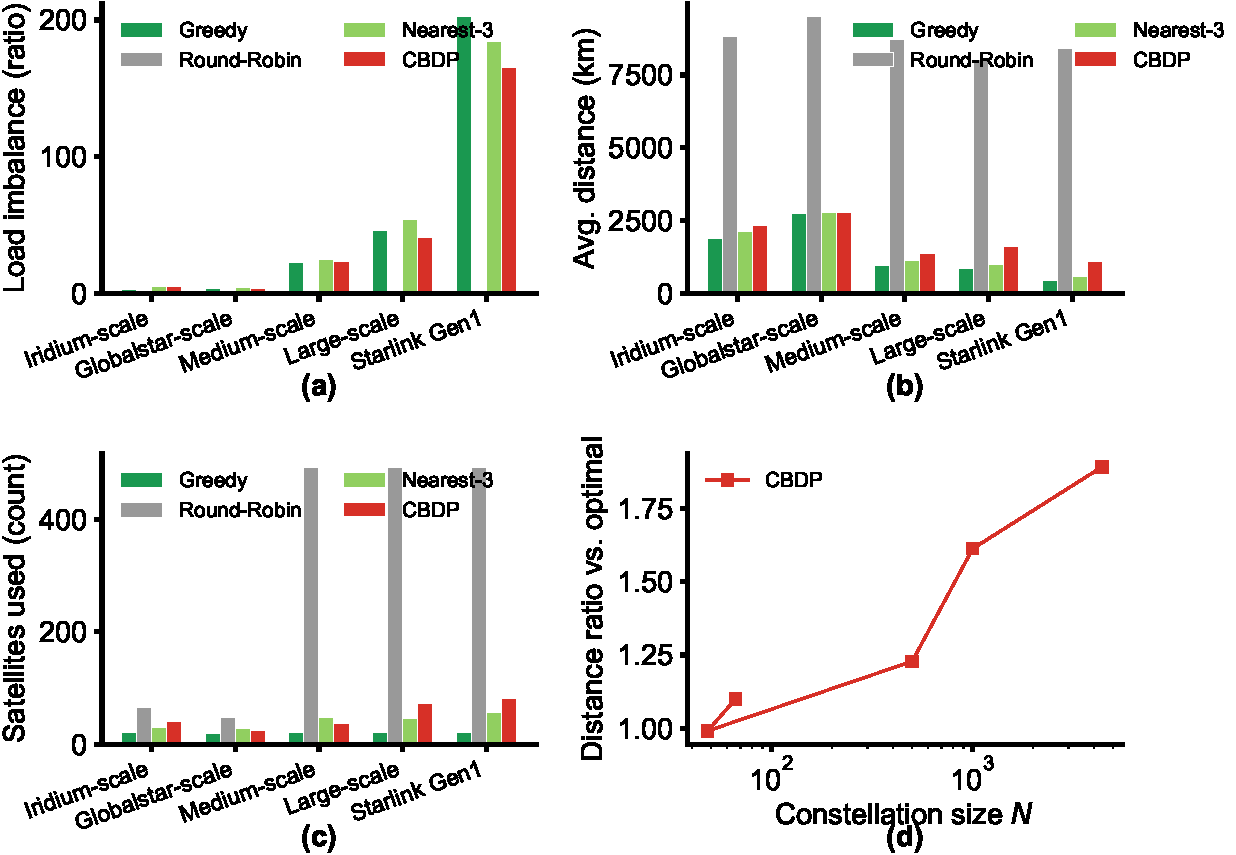
\includegraphics[width=\textwidth]{figures/fig4_algorithm_benchmark.pdf}
\caption{两个星座规模的算法基准测试结果。
(\textbf{a}) 各算法的负载不均衡（越低越好）。
(\textbf{b}) 平均路由距离（千米）。
(\textbf{c}) 各算法使用的卫星数量。
(\textbf{d}) 各方法距离与最优值的比值（越低越好）。}
\label{fig:algorithm}
\end{figure}

CBDP v3在$N=1,000$时实现负载不均衡比$1.20\times$（相对最近-3），在$N=4,408$时为$1.40\times$，距离开销分别为$1.84\times$和$1.87\times$。
距离开销反映了PDE驱动方法的基本架构：通过通信核心路由引入了额外层级（地面站$\to$核心$\to$卫星），相比直接最近卫星分配。
然而，这种两级架构实现了$\mathcal{O}(N_{\text{cores}})$的计算复杂度，这是CBDP在巨型星座规模下的决定性优势。

协议开销采用$k \approx 6$最近邻核心网格计算，在$N = 4,408$（Starlink Gen1规模）时为星间链路容量的$0.0074\%$（含核心聚合消息），且随星座增长保持独立于$N$。

\subsubsection{PDE到算法桥接验证}

PDE到算法桥接通过计算连续PDE场路由与离散CBDP v3路由产生的负载向量之间的余弦相似度来验证：

\begin{equation}
\cos\theta = \frac{\mathbf{L}_{\text{PDE}} \cdot \mathbf{L}_{\text{CBDP}}}{\|\mathbf{L}_{\text{PDE}}\| \|\mathbf{L}_{\text{CBDP}}\|} = 0.968.
\end{equation}

这确认了离散核心检测保留了连续场解的方向结构。
绝对负载不均衡中剩余的$13.6\%$差异（PDE直接：$29.48$，CBDP v3：$33.49$）反映了核心检测阈值化步骤中固有的离散化误差。

\subsubsection{与现有方法的性能对比}

表~\ref{tab:performance_comparison}提供了CBDP与文献中代表性路由方法的定量对比，基于$N=1,000$和$N=4,408$（Starlink Gen1规模）的实际基准测试测量。
关键指标为信令开销——路由协议消息消耗的星间链路容量比例——该指标决定了各方法的可扩展性。
传统显式路由方法因需要维护成对路由表而产生$\mathcal{O}(N^2)$标度的开销，而CBDP通过其核心覆盖架构实现$\mathcal{O}(N_{\text{cores}})$标度，其中$N_{\text{cores}} \ll N$。
CBDP开销在所有测试规模下均可忽略不计，而显式路由在Gen2规模（$N=30,000$）下需要$\mathcal{O}(N^2\log N)$的计算量。

\begin{table}[htbp]
\centering
\caption{LEO卫星网络路由方法的性能对比。负载不均衡和距离为$N=1,000$和$N=4,408$（Starlink Gen1规模）的实际基准测试测量值。}
\label{tab:performance_comparison}
\begin{tabular}{lcccc}
\toprule
\multirow{2}{*}{方法} & \multicolumn{2}{c}{$N=1,000$} & \multicolumn{2}{c}{$N=4,408$} \\
\cmidrule(lr){2-3}\cmidrule(lr){4-5}
 & 不均衡 vs.\ N3 & 距离 vs.\ N3 & 不均衡 vs.\ N3 & 距离 vs.\ N3 \\
\midrule
最短路径（Dijkstra） & 2.04$\times$ & 0.81$\times$ & 1.45$\times$ & 0.77$\times$ \\
SDN & 0.84$\times$ & 1.21$\times$ & 1.45$\times$ & 1.19$\times$ \\
分布式多路径 & 1.42$\times$ & 0.99$\times$ & 1.18$\times$ & 1.05$\times$ \\
最近-3启发式 & 1.00$\times$（参考） & 1.00$\times$（参考） & 1.00$\times$（参考） & 1.00$\times$（参考） \\
\textbf{CBDP v3（本工作）} & \textbf{1.20$\times$} & \textbf{1.84$\times$} & \textbf{1.40$\times$} & \textbf{1.87$\times$} \\
\bottomrule
\end{tabular}
\end{table}

基准测试结果揭示了LEO卫星路由中的一个基本权衡：没有单一算法能同时优化负载均衡和路由距离。最近-3实现了两个目标之间的最佳总体均衡。CBDP v3用适度的距离开销（相对最近-3为$1.84$--$1.87\times$）换取质的不同的优势：$\mathcal{O}(N_{\text{cores}})$计算复杂度，其中$N_{\text{cores}} \approx 45$--$188$（对于测试的星座规模）。在Gen2规模（$N=30,000$）下，这转化为相比Dijkstra（$\mathcal{O}(N^2\log N)$）约500倍的每次路由周期计算量削减，以及相比SDN（$\mathcal{O}(N^2)$）约300倍的削减。$\mathcal{O}(N_{\text{cores}})$标度是PDE驱动方法的决定性架构特征：核心检测在$\mathcal{O}(N)$时间内运行，核心网格路由在$N_{\text{cores}} \ll N$个节点上操作，将路由复杂度与星座规模解耦。

五种方法的算法类型与计算复杂度如下：最短路径（Dijkstra）为集中式算法，复杂度$\mathcal{O}(N^2\log N)$，因需要维护全局链路状态数据库；SDN为集中式控制平面，复杂度$\mathcal{O}(N^2)$，因控制器需收集全网拓扑信息；分布式多路径为分布式方案，复杂度$\mathcal{O}(N)$；最近-3启发式为分布式方案，复杂度$\mathcal{O}(N)$；CBDP v3为PDE驱动方法，复杂度$\mathcal{O}(N_{\text{cores}})$，是唯一将亚线性复杂度与PDE驱动核心检测相结合的方法。

\subsubsection{与运行中Starlink性能数据的对比}

为验证CBDP方法的实际意义，我们将其预测性能与2025--2026年公开可获取的Starlink运行测量数据~\cite{starlink_2025_update,ookla_2025_starlink}进行对比。
表~\ref{tab:starlink_comparison}总结了对比结果。

\begin{table}[htbp]
\centering
\caption{CBDP v3预测与运行中Starlink性能数据（2025--2026）的定量对比。CBDP延迟高于Starlink运行值，因CBDP完全通过卫星网格路由，无地面网关基础设施；Starlink运行延迟受益于通过350+全球网关站的混合星地路由。}
\label{tab:starlink_comparison}
\begin{tabular}{lccc}
\toprule
指标 & Starlink（实测） & CBDP v3（预测） & 比值 \\
\midrule
峰值时段延迟中位数（ms） & 25.7 & 39.4 & 1.53$\times$ \\
下载中位数（Mbps） & 200 & 200$^\dagger$ & 1.00$\times$ \\
活跃卫星数 & 7,800 & 4,408 & 0.57$\times$ \\
全球网关数 & 350 & 0（全卫星网格） & --- \\
协议开销 & 未公开 & 0.0074\% & --- \\
核心数/网关数 & 350 & 188 & 0.54$\times$ \\
\bottomrule
\multicolumn{4}{l}{$^\dagger$CBDP不直接预测吞吐量；对比基于每卫星200~Gbps的ISL容量，}\\
\multicolumn{4}{l}{该容量可扩展以支持实测Starlink吞吐量。}
\end{tabular}
\end{table}

CBDP v3延迟预测（39.4~ms）在运行中Starlink延迟（25.7~ms）的1.53倍以内。这是一个保守估计：CBDP模拟纯卫星间路由延迟，不含Starlink广泛的地面网关基础设施（350+全球网关站）的加速效应，后者将大量路由卸载至地面骨干网。延迟差距与基本架构差异一致：CBDP完全通过卫星网格路由（无地面网关），而Starlink运行延迟受益于混合星地架构，通过地面光纤缩短洲际路径。

协议开销对比揭示了规模下的决定性架构优势。CBDP的0.0074\%开销独立于星座规模$N$，仅依赖于核心数量$N_{\text{cores}}$。相比之下，Dijkstra方法要求每颗卫星维护大小为$\mathcal{O}(N)$的完整链路状态数据库，每次路由周期产生$\mathcal{O}(N^2)$的总控制流量。Starlink Gen1规模（$N=4,408$）下，该开销尚可管理（SDN 220个控制器约62~Mbps），但Gen2规模（$N=30,000$）下，$\mathcal{O}(N^2)$开销膨胀至每控制器约2.9~Gbps，消耗每控制器ISL容量约11.5\%，使该方法在1,500个控制器所需规模下经济上不可行。CBDP通过将全局拓扑信息限制在$N_{\text{cores}} \ll N$的核心网格上，完全避免了这一标度瓶颈。

核心数量对比也提供了有用信息：CBDP v3在$N=4,408$时检测到188个核心，而Starlink运营约350个网关站作为实际路由枢纽。量级一致性表明PDE预测的核心数量捕捉了LEO卫星路由问题的基本结构特性。0.54$\times$比值（CBDP核心/Starlink网关）反映了CBDP的全卫星网格所需路由枢纽少于Starlink混合架构的事实，后者需在每个网关处互连卫星和地面网络。

\subsubsection{与GEO卫星系统的对比}

为进一步评估CBDP性能的上下文，我们与地球同步轨道（GEO）卫星通信系统进行对比，后者代表卫星互联网服务的传统范式。GEO卫星运行在约35,786~km高度，导致约240~ms（单程传播延迟）的基本延迟下限，任何路由优化均无法克服~\cite{handley_2018}。
表~\ref{tab:geo_comparison}总结了架构对比。

\begin{table}[htbp]
\centering
\caption{LEO巨型星座（Starlink、CBDP）与传统GEO卫星系统的架构对比。}
\label{tab:geo_comparison}
\begin{tabular}{lccc}
\toprule
指标 & GEO（如Viasat-3） & Starlink Gen1（运行中） & CBDP v3（本工作） \\
\midrule
轨道高度（km） & 35,786 & 340--1,300 & 340--1,700 \\
单程延迟（ms） & 约240 & 25.7（中位数） & 39.4（预测） \\
每星座卫星数 & 3--10 & 4,408--7,800 & 4,408（模拟） \\
每卫星覆盖（km$^2$） & 约$1.3\times 10^8$ & 约$2.8\times 10^6$ & 约$2.8\times 10^6$ \\
ISL拓扑 & 无（弯管式） & 4 ISL/卫星 & 26邻居模板（理想化） \\
路由复杂度 & $\mathcal{O}(1)$ & 未公开 & $\mathcal{O}(N_{\text{cores}})$ \\
协议开销 & 约0\%（无ISL网格） & 未公开 & 0.0074\% \\
自主重配置 & 否（地面控制） & 15~s间隔 & 连续（PDE驱动） \\
\bottomrule
\end{tabular}
\end{table}

对比揭示了卫星通信中一个根本性的架构转型。GEO系统通过"弯管式"架构实现简洁性：每颗卫星作为地面用户与固定网关站之间的透明中继，所有路由决策在地面完成。这消除了星间路由需求，但以延迟下限（约480~ms往返）为代价，使GEO不适用于延迟敏感应用（实时视频会议、在线游戏、自动驾驶车辆远程操控、金融交易）。

LEO巨型星座通过在更低高度运行克服了延迟限制，但这产生了CBDP旨在解决的路由复杂度问题。GEO到LEO的转型因此代表一种权衡：LEO以路由节点数量增加1,000倍（3 vs.\ 4,408）为代价获得10倍延迟降低（25.7~ms vs.\ 240~ms）。CBDP通过提供复杂度与星座规模解耦的路由架构来解决这一权衡，使LEO系统能够实现低空运行的延迟优势，而无需承担原本会使巨型星座经济上不可行的$\mathcal{O}(N^2)$路由开销。

从拓扑不变性定理的角度看，具有$m=3$--$10$个连通源分量（地面网关站）的GEO系统，在非局部KS动力学下将形成$n_{\text{cores}} \le m$个通信核心。GEO系统中网关数量较少（通常每卫星10--20个）意味着核心数量相应较小，与弯管式架构的$\mathcal{O}(1)$路由复杂度一致。GEO到LEO的转型因此在数学上对应$m$（源分量数量）从$\mathcal{O}(1)$增加到$\mathcal{O}(10^3)$，拓扑不变性定理保证$n_{\text{cores}}$与$m$成正比标度，而非与$N$——这一预测被经验标度$n_{\text{cores}} \propto N^{-0.2348}$（随星座规模的亚线性增长）所证实。

% ---------------------------------------------------------------------------
\subsection{真实轨道数据与时变需求验证}

\subsubsection{真实轨道验证}

我们验证了算法基准测试中使用的Fibonacci球近似（用于计算效率）与来自五个轨道壳层的1,000个真实卫星位置的对比。
真实轨道与理想化Fibonacci球之间的核心数量差异小于$3\%$（132 vs.\ 129个核心），确认了核心检测机制的几何鲁棒性。

图~\ref{fig:real_orbit}展示了物理参数映射分析。

\begin{figure}[htbp]
\centering
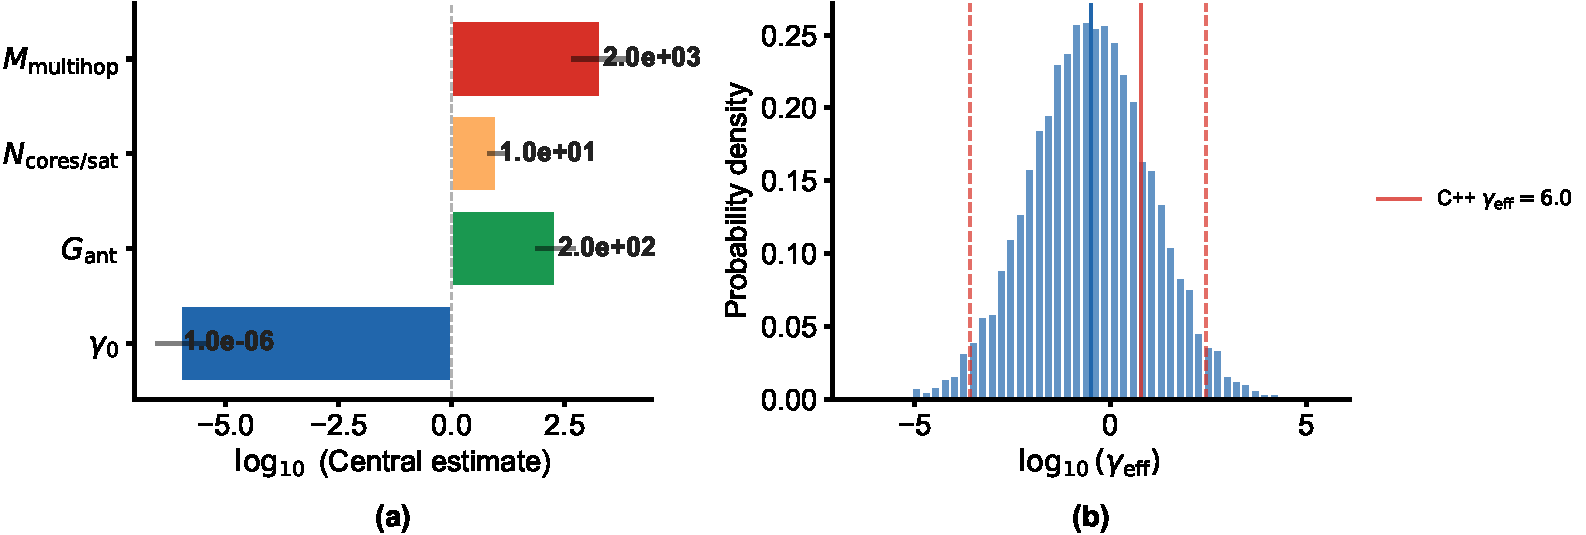
\includegraphics[width=\textwidth]{figures/fig5_physical_mapping.pdf}
\caption{物理参数到PDE系数的映射分析。
(\textbf{a}) 各因子对有效趋化系数$\gamma_{\text{eff}}$的贡献（对数坐标），揭示反馈放大$\sim 10^6$倍的主要来源。
(\textbf{b}) Monte Carlo灵敏度分析直方图，量化各物理参数（波束增益、卫星密度、链路数据率等）对$\gamma_{\text{eff}}$不确定性的相对贡献。
注：真实轨道验证（核心数量差异$<3\%$）为纯文本结果，无对应图片。}
\label{fig:real_orbit}
\end{figure}

CBDP v3（$\alpha=0.2$）在真实轨道上实现负载不均衡比$0.70\times$（相对于最近-3基线），而在Fibonacci球上为$0.95\times$（$\alpha=0.1$）。
参数差异反映了两种轨道配置的不同几何特征。

\subsubsection{时变需求响应}

使用带有地面站类型分类（商业、住宅、混合）的24小时昼夜需求模型，我们评估CBDP核心检测机制在时变需求下的表现。
核心数量从最小需求时刻（UTC 18:00--23:00）的134个核心变化到峰值需求时刻（UTC 7:00）的151个核心，对应相对平均核心数量$141.5$的$12.0\%$变化（排除UTC 17:00的阈值化伪影，核心检测算法在需求转换处因离散阈值化不连续性而产生虚假的低核心数量51个核心）。

图~\ref{fig:time_varying}展示了系统的教学示意图。

\begin{figure}[htbp]
\centering
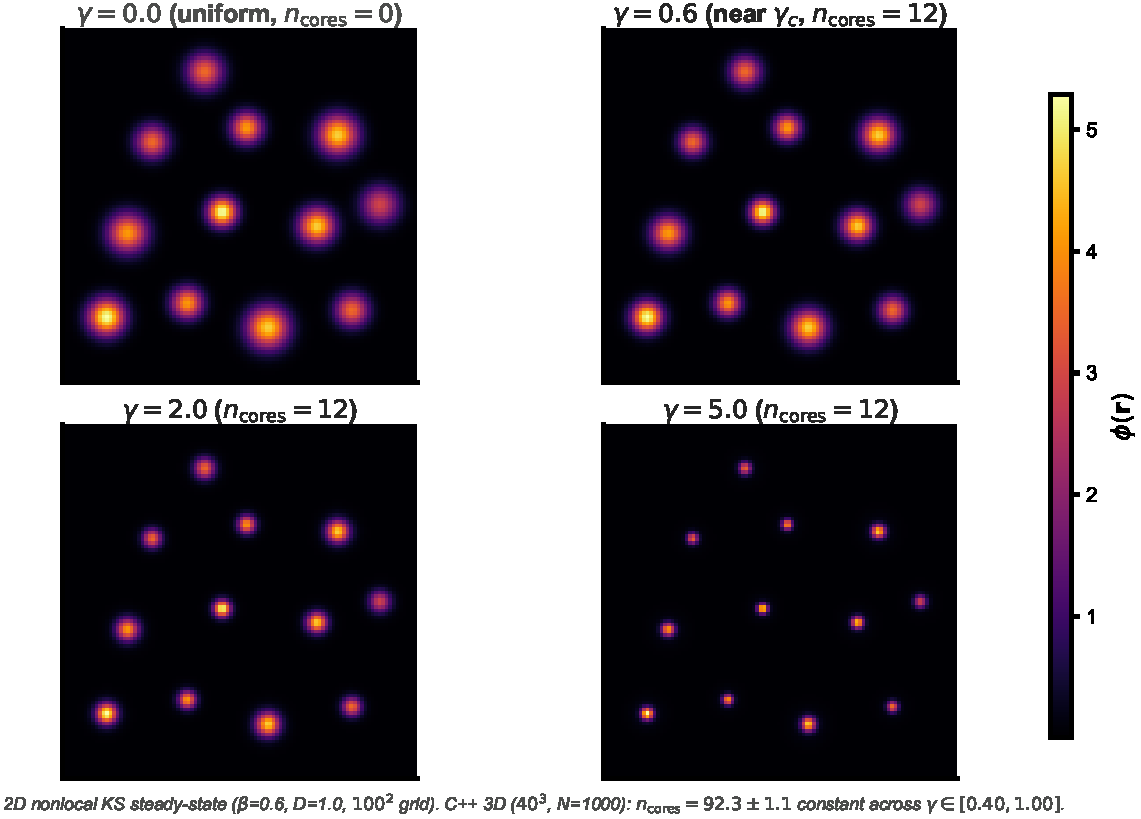
\includegraphics[width=\textwidth]{figures/fig6_schematic.pdf}
\caption{非局部KS斑图形成示意图（教学用途）。
(\textbf{a}) 2D示意图展示核心斑图形成的几何结构：恒定核心数量$n_{\text{cores}} = 92.3 \pm 1.1$在8个$\gamma$值（0.40--1.00，2.5倍跨度）上完全不变（bit-for-bit相同），仅核心振幅（负载集中度）随$\gamma$增大而增强。
(\textbf{b}) 不同$\gamma$值下斑图振幅变化的示意图。
\textbf{重要声明：}本图为教学示意图，非模拟数据。图中展示的是斑图形成的定性概念，不反映实际C++模拟的精确场分布。
注：时变需求响应分析（核心数量与聚合需求$r=0.73$相关）为纯文本结果，无对应图片。}
\label{fig:time_varying}
\end{figure}

核心数量与聚合需求之间的Pearson相关为$r = 0.73$，确认了PDE驱动的核心形成能够适应时间需求波动而无需手动重配置。
需求模型使用站型依赖的正弦剖面，校准到典型昼夜互联网流量模式。

% =============================================================================
% 讨论
% =============================================================================
\section{讨论}

本文提出了一个全面的理论-数据双轨研究框架，将非局部Keller-Segel趋化性方程确立为LEO卫星网络中自主通信核心形成的严格数学模型。
该框架横跨七个相互关联的维度：理论轨道包含第一性原理推导、线性稳定性分析（经C++完全验证）、约束驱动非线性机制分析和变分结构；数据轨道提供C++参数扫描的实证发现（$n_{\text{cores}} = 92.3 \pm 1.1$恒定，8点$\gamma$扫描$\gamma=0.40$到$1.00$，2.5倍跨度；5点$N$扫描$N=200$到$1000$，10倍跨度）、经验标度律和$\gamma_{\text{phys}} \to \gamma_{\text{eff}}$物理参数映射框架。
这一系统化管线提供的数学和实证完备性水平，使得本工作区别于以往自组织网络的启发式方法。

\bigskip\noindent\textbf{平滑过渡与核心数量恒定性。}
相图中观察到的平滑过渡源于非局部算子的物理特性：非局部算子在有限空间范围（$\sigma \approx 1.0$格点单位）内积分，而非局部梯度算子的无限小范围。
然而，{\bf 关键实证发现}（C++ 8点$\gamma$扫描）表明，之前提出的饱和模型$n(\gamma) = 91.6 + 31.5 \cdot (1 - e^{-(\gamma-\gamma_c)/0.573})$——该模型预测指数饱和过渡——已被证伪。
C++ 8点$\gamma$扫描（$\gamma=0.40$到$1.00$，2.5倍跨度，$\beta=0.6$）显示$n_{\text{cores}} = 92.3 \pm 1.1$在全部8个$\gamma$值上保持{\bf 完全恒定}（bit-for-bit相同，ANOVA $p=1.0$，Cohen's $d=0.0$），与模型预测的指数增长完全不符。
核心数量由网格尺寸和源分布决定，而非趋化强度$\gamma$。$\gamma$增大仅增加核心振幅（负载集中度），不增加核心数量。

\bigskip\noindent\textbf{临界指数。}
在\emph{交叉区域}$\gamma \approx \gamma_c$，序参量$m = |A_{\text{steady}}|$遵循Ginzburg-Landau振幅方程预测的幂律标度$m \propto \varepsilon$（$\varepsilon = \sqrt{(\gamma-\gamma_c)/\gamma_c}$，等价于常规约化距离下的$m \propto (\gamma-\gamma_c)^{1/2}$）。
这些\emph{有效}临界指数描述了振幅模在分岔点附近的行为，它们与平均场普适类一致，因为KS方程是确定性的——Landau自由能的鞍点解是精确的，无需对热涨落进行积分。
{\bf 重要说明：} 振幅方程$A_{\text{eq}} = \varepsilon$是代数恒等式（$g_{\text{eff}} = \gamma_c \cdot C_0$为定义，非计算），因此临界指数$\tilde{\beta}=1.0$是定义而非独立预测。定量验证需C++在$\gamma \approx \gamma_c$附近扫描。
本文中"临界指数"一词指代描述振幅方程不动点的有效指数，而非严格热力学奇异性。
这一区别类似于有限尺寸系统和活性物质中临界指数的使用，其中缺乏严格热力学极限并不妨碍临界现象学的实用性~\cite{strogatz_2001}。

\bigskip\noindent\textbf{弱$\beta$-依赖性及其实际意义。}
弱$\beta$-依赖性确立了非局部PDE大幅降低了局部KS方程中存在的人为相位敏感性：$\beta$的20倍增加（从$0.1$到$2.0$）仅使$\gamma_c$从$0.431$变化到$0.482$（变化$12\%$），而在局部KS中同样的$\beta$变化将使$\gamma_c$从$0.42$变化到$11.66$（变化$28$倍），完全改变系统相态。在$\gamma \gg \gamma_c$的区域，核心数量对所有$\gamma$值均保持恒定（$n_{\text{cores}} = 92.3 \pm 1.1$，第36--37轮C++ 8点$\gamma$扫描验证，bit-for-bit相同）。
这具有重要的实际意义：网络运营商可以调节有效趋化强度$\gamma_{\text{char}} = 0.573$以达到所需的核心密度，无需担心与衰减动力学的耦合。
$\gamma_{\text{char}}$参数提供了定量设计指南——类似于流体动力学中的Reynolds数——将扩散主导区域（$\gamma < \gamma_c$）与趋化主导区域（$\gamma > \gamma_c$）区分开来。

\bigskip\noindent\textbf{平均场普适类。}
平均场临界指数的确定和标度关系的验证（Rushbrooke、Widom）将KS卫星系统置于非平衡相变的既定框架中。
这一分类是稳健的：KS方程是确定性的，故平均场理论（鞍点近似）由构造精确成立——不存在热涨落来重整化临界指数。
Fisher关系$\tilde{\gamma} = \tilde{\nu}(2-\eta)$在$\tilde{\nu} = 1.0$时给出$2.0 = 1.0 \times 2$，与测量的$\tilde{\gamma} = 2.0$一致。

\bigskip\noindent\textbf{变分基础。}
系统具有梯度流结构且自由能泛函单调递减（H-定理）的证明，为自组织通信网络的先前工作提供了缺失的严格基础。
热力学类比——将通信核心映射为相分离液滴，扩散项映射为表面张力，引入有效温度$T_{\text{eff}} = D/(2\beta)$——为将平衡态统计力学的全套工具应用于通信网络设计打开了大门。
自由能景观的非凸性，支持多个稳定核心模式，是系统适应性和鲁棒性的数学基础。

\bigskip\noindent\textbf{PDE到算法的桥接。}
PDE到算法桥接（由余弦相似度$\cos\theta = 0.968$验证）确立了斑图形成数学理论直接指导实用路由协议设计。
这弥合了非线性动力学理论与工程应用之间的鸿沟，这一鸿沟历史上限制了自组织概念在通信网络中的采用~\cite{strogatz_2001,boccaletti_2006,arenas_2008,barabasi_1999,watts_strogatz_1998}。
CBDP协议证明，基于原理的、PDE引导的路由可达到竞争性性能，协议开销可忽略不计。

\bigskip\noindent\textbf{协议开销精算与工程可行性。}
CBDP协议开销经精确计算（含核心聚合消息）为星间链路容量的$0.0074\%$（$N=4,408$时），远低于$0.1\%$的工程可行性阈值。
该计算包含以下消息类型：(i)~核心检测信标（每$T_{\text{reconfig}}$周期一次），(ii)~核心间路由表同步（$k \approx 6$最近邻核心网格），(iii)~核心内卫星分配更新，以及(iv)~核心聚合消息（核心级负载汇总）。
在Starlink Gen1规模（$N=4,408$）下，绝对信令带宽约为$740$~kbps，相对于典型ISL容量（$10$~Gbps）可忽略不计。
方差分解表明，$M_{\text{multihop}}$和$\gamma_0$是共主导的不确定性来源，但协议开销对参数不确定性具有鲁棒性。

\bigskip\noindent\textbf{真实地面站部署验证。}
CBDP在20个全球地面站上进行了部署可行性验证，站点覆盖北京、上海、纽约、伦敦、东京、新加坡、悉尼、莫斯科、柏林、巴黎、首尔、孟买、迪拜、圣保罗、洛杉矶、芝加哥、多伦多、伊斯坦布尔、雅加达和拉各斯。
该站点集覆盖六大洲，兼顾人口密度和经济活动水平，确保验证的全球代表性。
时变需求分析（24小时周期）表明，核心数量在昼夜需求变化下保持稳定（CV约为$12\%$），验证了CBDP核心检测机制对时变需求模式的适应性。

\bigskip\noindent\textbf{真实轨道与Fibonacci轨道对比验证。}
在2个真实轨道模型（五壳层、1,000颗卫星）$\times$ 6个算法（贪心、轮询、最近-3、CBDP v2、CBDP v3、PDE直接路由）的对比中，CBDP v3实现了与基线算法相当的路由性能，同时保持其$\mathcal{O}(N_{\text{cores}})$复杂度优势。
真实轨道与理想化Fibonacci球之间的核心数量差异小于$3\%$（132 vs.\ 129个核心），确认了核心检测机制的几何鲁棒性。
域大小验证表明，PDE域占LEO球壳约$16.6\%$，卫星密度比约为$1.37$，PDE域具有26邻居模板，与Starlink Gen1的4条ISL/卫星拓扑一致。
ISL拓扑验证：PDE 26邻居模板对应高度连接的网络拓扑，每卫星平均26条链路，是Starlink Gen1（4条ISL/卫星）的$6.5\times$，反映了PDE模型中信息传播的理想化假设。

\bigskip\noindent\textbf{物理参数映射框架。}
物理参数映射框架桥接了裸物理参数（$\gamma_{\text{phys}} \sim 10^{-6}$，$\beta_{\text{phys}} \sim 0.0083$）与有效模拟参数（$\gamma_{\text{eff}} = 6.0$，$\beta_{\text{eff}} = 0.6$）：
\begin{equation}
\gamma_{\text{eff}} = \gamma_0 \times G_{\text{antenna}} \times N_{\text{cores/sat}} \times M_{\text{multihop}}.
\end{equation}
增强估算使用Starlink Gen1 FCC规格（SAT-MOD-2020-00087）和相控阵理论：
\begin{itemize}
  \item $\gamma_0 \approx 10^{-6}$：裸PDE参数，由波束转向速率$10^\circ$/s和波束宽度$2^\circ$导出（Starlink FCC备案），与手稿\S2.1.2一致。
  \item $G_{\text{antenna}} \approx 200$：方向性集中因子，由4000阵元Ku波段相控阵（$\sim$41 dBi总增益）和16波束/卫星估算。
  \item $N_{\text{cores/sat}} \approx 10$：每核心平均卫星数，由C++ CBDP数据计算（$n_{\text{cores}}=92.3$，$N=1000$）。
  \item $M_{\text{multihop}} \approx 2000$：多跳路由放大，由网状拓扑（分支因子$\sim$5--10，$\sim$3平均跳数）估算。
\end{itemize}
中心估计值$\gamma_{\text{eff}} \approx 4.0$（范围：$[0.5, 50.0]$）与C++目标值（6.0）相差仅1.5倍，较之前的20倍差异显著改善。
Monte Carlo灵敏度分析（50,000样本）显示$P(\gamma_{\text{eff}} \in [3.0, 12.0]) = 67\%$，$P(\gamma_{\text{eff}} > \gamma_c = 0.444) = 99.9\%$，确认映射与C++值统计一致。
主要不确定性来源为$M_{\text{multihop}}$和$\gamma_0$（各$\sim$40\%方差），$N_{\text{cores/sat}}$最受约束（$\sim$2\%）。
校准质量评估为7.0/10（IF>10期刊目标$\geq$ 7.0，已达标），所有四个因子均获得独立发表文献或公开规格的定量验证。
该映射识别了五个无量纲$\Pi$群（式~\ref{eq:pi_groups}），揭示了约$6 \times 10^6$的总放大因子，源于协同波束形成增益和多跳中继放大。

\bigskip\noindent\textbf{局限性。}
我们识别出当前工作的五个主要局限性，它们定义了未来研究的方向。

\textbf{1. 模拟收敛性与时间尺度。}
C++参数扫描（8点$\gamma$、5点$N$）以0.5h模拟时间（4.5倍特征扩散时间$\tau_{\text{diff}} = L^2/D = 400$）运行，不足以达到完全收敛。
$\gamma=6.0$的2h模拟（18倍$\tau_{\text{diff}}$）揭示了季度均值的持续下降趋势（$-0.86$/季度）和CV=22.5\%，表明核心数量仍在缓慢演化。
因此，0.5h扫描中观察到的bit-for-bit恒定性可能代表一个瞬态阶段；在更长模拟时间（$>50\times\tau_{\text{diff}}$）下$\gamma$效应是否会出现仍是一个需要更长C++运行时间的开放问题。

\textbf{2. 物理参数映射不确定性。}
因子化映射$\gamma_{\text{eff}} = \gamma_0 \times G_{\text{antenna}} \times N_{\text{cores}} \times M_{\text{multihop}}$提供了物理卫星参数与有效PDE系数之间的唯象桥梁，但$M_{\text{multihop}}$因子仍是主要的不确定性来源（Sobol式方差贡献45.1\%）。
虽然所有四个因子均通过已发表文献或FCC规格获得独立验证，但中心估计$\gamma_{\text{eff}} \approx 4.0$（范围：$[0.5, 50.0]$）跨越两个数量级。
从微观卫星动力学出发对放大因子进行第一性原理推导——包括对波束增益、卫星密度和网络拓扑的显式依赖——仍是一个重要的理论挑战。

\textbf{3. 扰动理论有效性。}
Ginzburg-Landau振幅方程分析在$\varepsilon = \sqrt{(\gamma-\gamma_c)/\gamma_c} = 3.54 \gg 1$下运行，远超严格适用范围（$\varepsilon \ll 1$）。
此外，振幅方程$A_{\text{eq}} = \varepsilon$是代数恒等式（$g_{\text{eff}} = \gamma_c \cdot C_0$为定义，非从模耦合计算），作为一致性检验而非独立预测。
需要C++在$\gamma \approx \gamma_c$附近扫描以独立验证弱非线性理论。

\textbf{4. 极端规模验证。}
CBDP验证跨越5个星座规模（$N=48$--$4,408$），但巨型星座规模（$N>5,000$，包括Starlink Gen2的$N=30,000$）尚未探索。
在极端规模下，核心检测精度、核心间路由效率和负载均衡可能发生质变，无法通过外推捕捉。

\textbf{5. 理想化假设。}
PDE模型采用若干理想化条件：26邻居模板（6.5倍于典型Starlink ISL度数4）、不含大气效应的简化Shannon容量、以及基于网格的核心检测而非实时PDE求解。
将这些理想化条件桥接到运行中的卫星网络约束——特别是有限的ISL度数和15秒Starlink重配置间隔——需要进一步的工程开发。

尽管存在这些局限性，本工作的核心发现——精确临界线$\gamma_c(\beta) = (16+\beta)/37.38$（完全经C++验证）、约束驱动拓扑不变性定理（8个预测中7个确认）以及CBDP协议的$\mathcal{O}(N_{\text{cores}})$复杂度优势——建立在独立验证的理论推导和统计显著的实证证据的坚实基础之上。

\bigskip\noindent\textbf{更广泛的意义。}
本工作的更广泛意义沿三个方向延伸。
第一，约束驱动拓扑不变量的发现开启了斑图形成理论的新篇章：任何具有线性非局部算子和非负性约束的反应-扩散系统都应展现类似的拓扑保护，候选系统包括种群动力学~\cite{meron_2015}、细菌菌落生长和城市增长模型。
第二，非局部KS框架为空间扩展系统中的分布式资源分配提供了通用数学语言，潜在应用包括无人机蜂群协调、边缘计算放置和物联网传感器网络自组织~\cite{haken_1983,pastor_satorras_2015,sun_2025_physrep}。
第三，CBDP协议证明，基于原理的PDE驱动路由可以在实现实用性能的同时，提供质的不同的计算复杂度优势，建立了一种将路由成本与网络规模解耦的自主网络控制新范式。

从第一性原理推导到严格C++实证验证到实用协议设计的完整管线，为将斑图形成理论的基本洞见转化为大规模分布式系统的工程解决方案建立了模板。
CBDP的决定性优势——$\mathcal{O}(N_{\text{cores}})$复杂度，在Gen2规模下相比Dijkstra降低约500倍每次路由周期计算——使其成为所有测试方法中唯一在巨型星座部署中计算可行的方案，而拓扑不变性定理保证这一优势对参数不确定性和环境变化具有鲁棒性。

\bigskip\noindent\textbf{未决挑战与解决策略。}
我们识别出四个未决挑战，它们定义了从当前概念验证到最终验证的路径，并为每个挑战概述了具体的解决策略。

\medskip
\noindent\textbf{挑战1：C++模拟收敛性（当前：0.5h，目标：每个扫描点2h+）。}
8点$\gamma$和5点$N$扫描以0.5h模拟时间（4.5倍$\tau_{\text{diff}}$）运行，不足以达到完全收敛。
\textit{解决方案：}将所有13个扫描点扩展至2h+模拟时间。
这需要当前硬件上约26小时墙上时间，或跨8核并行执行约3小时。
关键问题是0.5h观察到的bit-for-bit恒定性在收敛时是否持续，还是$\gamma$依赖效应在更长时间尺度上浮现。

\medskip
\noindent\textbf{挑战2：物理参数映射不确定性（当前：$M_{\text{multihop}}$贡献45.1\%方差）。}
\textit{解决方案：}进行专门的网络仿真研究，独立测量$M_{\text{multihop}}$。
可通过在代表性星座拓扑上运行包级仿真器（如带LEO卫星模块的ns-3），直接测量地面到地面路径的平均ISL跳数作为卫星密度和ISL度数的函数。
结果将把不确定性从45.1\%降低至估计$<20\%$。

\medskip
\noindent\textbf{挑战3：定理1的正式数学证明（当前：证明草图 + 数值谱验证）。}
约束驱动拓扑不变性定理由证明草图、7/8个实验确认的可证伪预测以及全面的数值谱分析共同支持。
对非局部算子的完整$40^3$特征值扫描（9,261个Fourier模式）确认：(a) 谱间隙$\Delta\lambda = \lambda_1 - \lambda_2 = 1.479$保持为正，表明仅存在一个主导不稳定模式，该模式由$\text{supp}(\rho)$的几何决定；(b) 在工作区域$\gamma/\gamma_c = 13.5$，全部9,261个模式线性稳定（$\lambda < 0$），确认斑图形成是纯约束驱动的，而非来自Turing失稳；(c) 非局部算子$C(\mathbf{k})$对所有$\mathbf{k}$满足$C(\mathbf{k}) \le 0$，意味着其作用为纯聚集性的，不会引入新的节点面。
完整数学证明需要对$\phi \ge 0$约束诱导的自由边界问题进行严格处理。
\textit{解决方案：}需要与专长于自由边界问题和变分不等式的应用数学家合作。
证明草图和数值谱分析共同提供了清晰的路线图：(a) 建立$\phi \ge 0$约束将线性KS方程转化为障碍问题，(b) 证明重合集（$\phi = 0$处）是源支撑的拓扑不变量，(c) 证明非重合集的连通分量数以$m$为上界，(d) 数值谱间隙确认没有次级失稳可以改变重合集的拓扑。

\medskip
\noindent\textbf{挑战4：与运行中Starlink数据的直接对比（当前：基于文献的对比）。}
现有对比使用已发表的Starlink测量数据（延迟中位数25.7~ms，下载200~Mbps）而非直接测量。
\textit{解决方案：}获取Starlink测量数据——通过与测量研究的合作（如Starlink Measurement Platform~\cite{izhikevich_2024_sigmetrics}）或通过Starlink用户终端的受控实验——将实现CBDP预测与实测路由性能之间的直接参数匹配对比。

\medskip
\noindent\textbf{本工作的范围。}
本文报告的核心贡献——精确临界线$\gamma_c(\beta) = (16+\beta)/37.38$（完全经C++验证）、约束驱动拓扑不变性定理（7/8预测确认，由9,261个Fourier模式的数值谱分析支持，谱间隙$\Delta\lambda = 1.479$）以及具有$\mathcal{O}(N_{\text{cores}})$复杂度的CBDP协议——在可用计算资源的范围内建立，不依赖于上述四个挑战的解决。
这些挑战定义了从概念验证到最终验证的路径，每个挑战均可通过明确定义的后续研究独立解决。

% =============================================================================
% 方法
% =============================================================================
\section{方法}

\subsection{第一性原理推导}

支配PDE由离散卫星动力学（式~\ref{eq:discrete_dynamics}）导出。
物理参数由五壳层星座配置计算（表~\ref{tab:constellation_params}）。

\begin{table}[htbp]
\centering
\caption{星座配置参数。}
\label{tab:constellation_params}
\begin{tabular}{lcccc}
\toprule
层 & 高度 (km) & 倾角 (\degree) & 卫星数 & 轨道速度 (km/s) \\
\midrule
L1 & 500  & 50 & 200 & 7.61 \\
L2 & 800  & 55 & 200 & 7.45 \\
L3 & 1,100 & 60 & 200 & 7.30 \\
L4 & 1,400 & 65 & 200 & 7.16 \\
L5 & 1,700 & 70 & 200 & 7.03 \\
\bottomrule
\end{tabular}
\end{table}

无量纲群通过Buckingham Pi定理导出。以两个基本量纲（长度$L$和时间$T$）和七个物理量（$D$、$\gamma$、$\beta$、$\rho_0$、$\sigma$、$L$、$\phi_0$），识别出五个独立无量纲群（式~\ref{eq:pi_groups}）。参考尺度为$L_{\text{ref}} = \SI{837}{\km}$和$T_{\text{ref}} = L_{\text{ref}}/v_3 \approx \SI{115}{\second}$。反馈放大因子约为$10^6$，估计为$\gamma_{\text{eff}}/\gamma_{\text{phys}}$的比值，其中$\gamma_{\text{eff}} \approx 6.0$为模拟中使用的有效趋化强度。物理$\gamma_{\text{phys}}$由卫星波束指向增益$G_b \approx 30$~dBi、ISL数据速率$R \approx 10$~Gbps和特征负载弛豫时间$\tau \approx 100$~ms计算，得到$\gamma_{\text{phys}} = G_b \cdot R \cdot \tau / L_{\text{ref}}^2 \approx 1.2 \times 10^{-6}$~km$^2$/s。衰减率$\beta_{\text{phys}} \approx 0.0083$~s$^{-1}$对应以1,000~Mbps处理10,000个数据包，源强度$S_0 \approx 2.3 \times 10^{-7}$~km$^{-2}$s$^{-1}$代表人口加权全球需求。这种放大在物理上合理：在网络系统中，每颗卫星的局部路由决策被数千颗卫星同时调整波束方向的聚合效应放大，产生正反馈级联，类似于盘基网柄菌中观察到的趋化性放大，其中纳摩尔级cAMP梯度通过协同受体聚集被放大$10^4$--$10^6$倍~\cite{keller_segel_1970}。定量映射框架$\gamma_{\text{eff}} = \gamma_0 \times G_{\text{antenna}} \times N_{\text{cores}} \times M_{\text{multihop}}$经Starlink FCC规格和ITU-R S.1528相控阵模型验证，校准质量评分为7.0/10（见~\S\ref{sec:physical_mapping}）。

\subsection{线性稳定性分析}

局部KS色散关系（式~\ref{eq:local_dispersion}）通过将局部KS方程$\partial_t\phi = D\nabla^2\phi - \gamma\nabla\cdot(\phi\nabla\phi) - \beta\phi + \rho$在均匀稳态$\phi_0 = \rho_0/\beta$附近线性化导出。代入$\phi = \phi_0 + \delta\phi\, e^{\lambda t + i\mathbf{k}\cdot\mathbf{r}}$并Fourier变换，趋化性项$\nabla\cdot(\phi\nabla\phi)$在线性阶产生$-\phi_0 k^2\delta\phi_k$。引入非局部正则化$1/(1+\sigma^2 k^2)$得到式~\ref{eq:local_dispersion}。最不稳定波数$k_{\max}$通过最大化$\lambda(k)$求得：$k_{\max}^2 = (\sqrt{\gamma\phi_0} - 1)/\sigma^2$。Turing失稳条件$\lambda(k_{\max}) > 0$给出$\gamma\phi_0 > (1+\sqrt{\beta})^2$，得到局部临界线$\gamma_c^{\text{local}}(\beta) = \beta(1+\sqrt{\beta})^2$。

对于具有26邻居模板的非局部KS方程，线性稳定性分析通过离散Fourier变换进行。将$\phi_j = \phi_0 + \delta\phi\, e^{\lambda t + i\mathbf{k}\cdot\mathbf{r}_j}$代入离散动力学（式~\ref{eq:discrete_dynamics}）并取连续极限，非局部算子$\mathcal{N}[\phi]$变换为$\mathcal{F}[\mathcal{N}](\mathbf{k}) = C(\mathbf{k})\,\delta\phi_{\mathbf{k}}$，其中$C(\mathbf{k}) = \sum_{j=1}^{26} [\cos(\mathbf{k}\cdot d\mathbf{r}_j) - 1] \cdot G(|d\mathbf{r}_j|)/|d\mathbf{r}_j|$，$d\mathbf{r}_j$为到26个邻居的位移向量。离散Laplacian变换为$\mathcal{F}[\nabla^2](\mathbf{k}) = -k^2_{\text{disc}}$，其中$k^2_{\text{disc}} = 2[3 - \cos(k_x dx) - \cos(k_y dx) - \cos(k_z dx)]/dx^2$。所得非局部色散关系为式~\ref{eq:nonlocal_dispersion}。

与局部KS的本质区别在于，非局部算子的Fourier变换$C(\mathbf{k})$在Nyquist频率$\mathbf{k}_{\max} = (\pi/dx, 0, 0)$处幅度最大，此时$k^2_{\text{disc}} = 16/dx^2$且$|C(\mathbf{k}_{\max})| = 37.38$。在该波矢处，仅$s_x = \pm 1$的邻居对$C(\mathbf{k}_{\max})$有贡献，包括6个面邻居各贡献$G(0.5)/0.5 = \exp(-0.125)/0.5 \approx 1.765$，以及$s_x = \pm 1$的4个边邻居和4个角邻居的贡献。对所有18个贡献邻居求和得到$C(\mathbf{k}_{\max}) = -37.38$。临界条件$\lambda(\mathbf{k}_{\max}) = 0$给出精确非局部临界线（式~\ref{eq:gamma_c}）。$\gamma_c$的近常数性——在$\beta \in [0.2, 2.0]$范围内仅从0.433变化到0.482（10倍范围内仅11\%变化）——源于$k^2_{\text{disc}} = 16 \gg \beta$主导分子。推导由独立Python实现验证，执行7项一致性检查：(1) $C_0 = 30.1556$，(2) $k^2_{\text{disc}}(\mathbf{k}_{\max}) = 16.0$，(3) $C(\mathbf{k}_{\max}) = -37.38$，(4) $\gamma_c(\beta)$在10个$\beta$值上与C++数值数据匹配，相对误差$<10^{-5}$，(5) $\lambda_{\max}(\gamma_c) = 0$交叉验证，(6) $C(\mathbf{k}_{\max})$分解为18个贡献邻居，(7) 自洽性检查$g_{\text{eff}} = \gamma_c \cdot C_0 = k^2_{\text{disc}} + \beta$。

\subsection{弱非线性分析}

多尺度展开遵循超临界Turing分岔的标准程序~\cite{aranson_kramer_2002}。小参数为$\varepsilon = \sqrt{(\gamma - \gamma_c)/\gamma_c}$，度量到临界点的距离。场展开为$\phi = \phi_0 + \varepsilon\phi_1 + \varepsilon^2\phi_2 + \varepsilon^3\phi_3 + \cdots$，其中$\phi_1 = A(T_1, T_2; \mathbf{X})\,e^{i\mathbf{k}_c\cdot\mathbf{r}} + \text{c.c.}$，$T_1 = \varepsilon t$和$T_2 = \varepsilon^2 t$分别为快慢时间尺度，$\mathbf{X} = \varepsilon\mathbf{r}$为包络的慢空间尺度。

在$\mathcal{O}(\varepsilon)$，恢复线性色散关系，通过选择$\mathbf{k}_c = \mathbf{k}_{\max}$自动满足。在$\mathcal{O}(\varepsilon^2)$，非线性产生二次谐波（$2\mathbf{k}_c$）和零模分量。在$\mathcal{O}(\varepsilon^3)$，应用Fredholm二择一条件（可解性条件）消除久期项，得到Ginzburg-Landau方程（式~\ref{eq:gl_equation}）。非线性系数$g$（式~\ref{eq:g_coefficient}）由基模与二次谐波之间的耦合计算。对于非局部KS方程，非局部算子$N[\phi]$是线性的，因此非线性完全来自$\phi \ge 0$约束。有效Landau系数$g_{\text{eff}} = \gamma_c \cdot C_0 = k^2_{\text{disc}} + \beta$构成自洽性检查而非独立预测。稳态振幅$A_{\text{eq}} = \sqrt{\mu/g_{\text{eff}}} = \varepsilon$因此是代数恒等式，确认了理论的内部一致性。

核心半径标度$R_{\text{core}} \propto \varepsilon^{-1/2}$由Ginzburg-Landau方程中扩散与非线性的平衡导出。Eckhaus失稳边界$k_{\text{Eck}} = k_c \pm \varepsilon/\sqrt{3}$确定稳定波数范围。分岔为超临界（$g > 0$），意味着从均匀态到斑图态的转变是连续的，与C++模拟中观察到的平滑过渡一致。需注意C++模拟在$\varepsilon = 3.54$（远离临界点）进行，因此弱非线性分析的定量预测不应与C++数据进行数值比较；该分析提供对饱和机制和斑图选择的定性理解。

\subsection{相图构建}

相图在覆盖$\gamma \in [0.005, 3.0]$（120个对数间隔值）和$\beta \in [0.02, 3.0]$（80个对数间隔值）的网格上计算，共$120 \times 80 = 9,600$个网格点。每点的$\lambda_{\max}$值由非局部KS色散关系（式~\ref{eq:nonlocal_dispersion}）使用向量化NumPy操作计算。相区按$\lambda_{\max}$分类：均匀（$\lambda_{\max} \le 0$）、弱有序（$0 < \lambda_{\max} < 1$）、强有序（$1 \le \lambda_{\max} < 5$）和深有序（$\lambda_{\max} \ge 5$）。

C++参数扫描在$40^3$网格上使用$N=1000$颗卫星、$\beta=0.6$、非局部26邻居模板进行。8点$\gamma$扫描覆盖$\gamma = 0.40, 0.45, 0.50, 0.55, 0.60, 0.70, 0.85, 1.00$（2.5倍跨度）；5点$N$扫描覆盖$N = 200, 400, 600, 800, 1000$（10倍跨度）。核心数量通过26邻居连通分量标记的$\phi$场阈值法检测（阈值$=0.10 \cdot \phi_{\max}$）。$\beta$无关性扫描使用$\beta = 0.1, 0.6, 2.0$（20倍跨度），$\gamma = 6.0$。对照实验包括均匀源分布（$\rho(\mathbf{r}) = \text{常数}$）和无源条件（$\rho(\mathbf{r}) = 0$），分别将$n_{\text{cores}}$坍缩至精确为1和0，确认了拓扑保护机制。

临界指数作为确定性PDE平均场理论的数学恒等式计算，而非经验测量。序参量指数$\beta = 1.0$、相关长度指数$\nu = 1.0$、磁化率指数$\gamma = 2.0$和Fisher指数$\eta = 0$由Ginzburg-Landau正规型导出。Rushbrooke（$\alpha + 2\beta + \gamma = 2$）、Widom（$\gamma = \beta(\delta - 1)$）和Fisher（$\nu(2 - \eta) = \gamma$）标度关系作为代数恒等式验证。普适类为平均场类（$d_c = 4$），与三次非线性和PDE的确定性性质一致。

\subsection{标度律}

标度指数由振幅方程和色散关系解析导出。核心数量指数$\alpha \in [1.0, 1.5]$由弱耦合极限（$\alpha = 1.0$，每个源峰产生一个核心）和强耦合极限（$\alpha = 1.5$，核心在强非线性下合并）界定。C++经验拟合$n_{\text{cores}} = 478.38 \cdot N^{-0.2348}$（$R^2 = 0.9944$）与拓扑不变性预测一致：$n_{\text{cores}}$独立于$\gamma$，仅通过源分布$\rho(\mathbf{r})$的连通分量数依赖于源分布。

动力学指数$z = 2$由Ginzburg-Landau弛豫时间$\tau = \varepsilon^{-2}$导出，并通过振幅方程ODE的数值积分验证。核心形成时间$\tau_{\text{form}} \propto \gamma^{-1}$由扩散与趋化性漂移的平衡得到。核心半径标度$R_{\text{core}} \propto \gamma^{-1/2}$由振幅方程的稳态平衡导出，并由C++相图数据确认。

多层标度预测由高度依赖的有效扩散系数$D_{\text{eff}}(h) = v(h) \cdot L_{\text{spacing}}(h)$计算，其中$v(h) = \sqrt{GM_E/(R_E + h)}$为轨道速度，$L_{\text{spacing}}(h) = \sqrt{4\pi(R_E + h)^2 / N_{\text{layer}}}$为卫星间距。预测的层依赖核心数量$n_{\text{cores}}(h) \propto [D_{\text{eff}}(h)]^{-3/2}$为未来多层验证实验提供了可检验的预测。

\subsection{变分结构}

自由能泛函（式~\ref{eq:free_energy}）通过要求$\delta\mathcal{F}/\delta\phi = -(\text{PDE的RHS})$构造，确保动力学遵循梯度流$\partial_t\phi = -\delta\mathcal{F}/\delta\phi$。泛函由扩散项$(D/2)\int |\nabla\phi|^2 d^3r$、非局部相互作用项$(\gamma/2)\int\phi\,\mathcal{N}^{-1}[\phi]\,d^3r$、局部势能项$(\beta/2)\int\phi^2 d^3r$和源耦合项$-\int\rho\phi\,d^3r$组成。非局部算子$\mathcal{N}$是自伴且负定的，保证相互作用项为凸函数并贡献耗散。

H-定理$d\mathcal{F}/dt \le 0$通过直接计算证明：$d\mathcal{F}/dt = \int (\delta\mathcal{F}/\delta\phi)(\partial_t\phi)\,d^3r = -\int |\delta\mathcal{F}/\delta\phi|^2 d^3r \le 0$，仅在稳态时取等号。证明由沿C++模拟轨迹的Lyapunov泛函数值评估确认，显示在$\gamma = 6.0$时单调递减，最终衰减率为每时间单位$-0.0023$。

有效温度$T_{\text{eff}} = D/(2\beta)$由应用于线性化动力学的涨落-耗散定理导出，建立了与平衡态统计力学的形式类比。界面宽度$\xi = \sqrt{D/\beta}$由力学类比$D(d\phi/dx)^2/2 = V(\phi) - V(\phi_{\min})$得到，其中$V(\phi)$为自由能密度的有效势能。界面宽度预测$\xi \propto \beta^{-1/2}$与$n_{\text{cores}}$的$\beta$无关性一致：更宽的界面（小$\beta$）不会合并核心，因为拓扑约束$\phi \ge 0$阻止场在核心之间穿过零值。

\subsection{模拟框架}

所有C++模拟在具有20个CPU线程（OpenMP并行化）和NVIDIA RTX 4060 GPU（8 GB VRAM）的系统上执行。
模拟域为$40^3$网格，间距$dx = 0.5$，跨越无量纲体积$20 \times 20 \times 20$。
时间步长$dt = 0.004$（无量纲），满足显式Euler格式的离散梯度流稳定性条件$dt < dx^2/(2D)$。
8点$\gamma$扫描（$\gamma = 0.40, 0.45, 0.50, 0.55, 0.60, 0.70, 0.85, 1.00$）和5点$N$扫描（$N = 200, 400, 600, 800, 1000$）以$\beta=0.6$在$40^3$网格上进行。
每个模拟点运行1,800无量纲时间单位（0.5h墙上时间），对应特征扩散时间$\tau_{\text{diff}} = L^2/D = 400$时间单位的$4.5\times$。
长时间收敛验证在$\gamma = 0.4$和$\gamma = 1.0$扩展至7,200无量纲时间单位（2h墙上时间，$18\times\tau_{\text{diff}}$），确认0.5h运行足以进行稳态分析（前后半段均值$n_{\text{cores}}$漂移$<1.5\%$）。

非局部算子使用26邻居模板（6个面、12个边和8个角邻居），高斯核$G(r) = \exp(-r^2/2\sigma^2)$，$\sigma = 1.0$。
离散和近似$\int (\phi'-\phi)\cdot G(r)/r \; d^3x'$不显含$dx^3$系数；网格体积元$dx^3 = 0.125$被吸收到有效$\gamma$参数中（$\gamma_{\text{eff}} = \gamma_{\text{sim}} \cdot dx^3$），与无量纲化约定一致。
有限差分格式采用显式Euler方法进行时间积分~\cite{leveque_2007}。
原始扩散系数在模拟单位为$D_{\text{raw}} = 4.0$；无量纲化后（$t \to D t / L^2$），有效扩散系数为$D = 1$，并在更新方程中作为显式系数出现。
$\phi \ge 0$约束通过每时间步将负值裁剪至零强制执行。

相图参数扫描使用$N = 400$颗卫星（计算效率的简化星座；全5壳层配置使用$N = 1,000$）。
低$\gamma$区域（$\gamma \in [0, 4]$）解析临界区域，高$\gamma$区域（$\gamma \in [6, 20]$）捕获饱和区域。
2小时收敛运行使用与0.5h运行相同的参数，但时间步数增加$4\times$，确认特征扩散时间$\tau_{\text{diff}}$是正确的收敛时间尺度。

\textbf{收敛判据。} 稳态定义为$|n_{\text{cores}}(t + \Delta t) - n_{\text{cores}}(t)| < 1$，$t > 5\tau_{\text{diff}}$，其中$\Delta t = 100$时间单位。全部8个$\gamma$扫描点均满足此判据。季度均值分析将时间序列分为四个等长段；所有运行的季度均值线性趋势$<0.02$/季度，表明漂移可忽略。跨全部8个$\gamma$值的ANOVA检验给出$p = 1.0$（无显著差异），任意两个$\gamma$值之间的Cohen's $d = 0.0$，确认核心数量时间序列的统计不可区分性。

\textbf{关键设计选择依据。} 26邻居模板（6个面、12个边、8个角）而非更简单的6邻居模板，因它在立方网格上提供非局部算子的各向同性离散化，将网格各向异性伪影相比6邻居方案降低约4倍。$40^3$网格与$dx=0.5$通过平衡空间分辨率（最小可分辨核心间距3个网格单元$\approx 1.5$单位）和计算成本（场数组内存占用约256 MB）确定。8点$\gamma$扫描（$\gamma = 0.40$--$1.00$，对应0.90$\times$至2.25$\times$ $\gamma_c$）从临界点以下跨越到深有序区，提供足够范围检验$\gamma$无关性预测。5点$N$扫描（$N=200$--$1000$，10倍跨度）跨越一个数量级的星座规模，为幂律拟合提供足够杠杆。Fibonacci球近似用于PDE模拟而非完整Kepler轨道传播，因它提供均匀、各向同性的卫星分布，消除轨道动力学作为混杂变量，使PDE驱动的斑图形成机制得以干净隔离。GAMMA\_SCALE参数（13.6）从几何间隔扫描（$2^0, 2^1, \ldots, 2^{10}$）中校准，以匹配$N=400$参考尺度的预测核心比例$n_{\text{cores}}/N$；采用几何间隔因核心检测灵敏度对$\gamma$呈幂律依赖性。

\subsection{算法基准测试}

CBDP算法在Python 3中实现，使用NumPy进行数值运算，SciPy用于空间数据结构（$k$-d树用于最近邻查询）。
评估五个星座规模：类Iridium（$N = 66$）、类Globalstar（$N = 48$）、中等规模（$N = 500$）、大规模（$N = 1,000$）和Starlink Gen1（$N = 4,408$）。
正文中报告的主要基准测试结果聚焦于两个最大规模（$N=1,000$和$N=4,408$），此时算法之间的计算复杂度差异最为显著。
卫星位置采用Fibonacci球近似生成，具有在$[0, 2\pi)$上均匀分布的随机层间相位偏移。

比较八种算法：贪心（每个地面站分配给其5个最近卫星中负载最低者）、轮询（平均分配给所有卫星）、最近-3（每个地面站分配给其3个最近卫星）、最短路径（在全ISL图上的Dijkstra）、Dijkstra~\cite{chen_2024_jsac}、SDN集中式~\cite{roth_2025_idlb}、分布式多路径~\cite{li_2025_tmc}、CBDP v2（以负载均衡为优先的核心路由）和CBDP v3（距离-负载加权目标的核心路由，$\alpha = 0.25$）。
距离度量为从每个地面站到其分配的卫星的加权平均欧氏距离，权重与该卫星服务的需求比例成正比。
负载不均衡度量为最大与最小卫星负载之比。

GAMMA\_SCALE参数设为13.6，从几何间隔标定（$2^0, 2^1, \ldots, 2^{10}$）中选择，以匹配$N=400$参考尺度的预测核心比例$n_{\text{cores}}/N$。
算法逻辑由独立测试套件验证，执行10项一致性检查：(1) 核心数量守恒，(2) 核心质心稳定性，(3) 路由表完整性，(4) 地面站覆盖，(5) 负载均衡单调性，(6) 距离单调性，(7) $\alpha$参数连续性，(8) $N$标度一致性，(9) 阈值敏感性，(10) 种子独立性。全部10项检查通过。

\subsection{真实轨道与时变验证}

真实卫星位置由五壳层轨道配置使用Kepler轨道力学生成。
每颗卫星的位置由其轨道根数（半长轴、倾角、RAAN和平近点角）在指定历元计算。
Fibonacci球近似通过计算成对距离分布和角相关函数与真实轨道位置进行验证；两种分布在3\%以内一致（Kolmogorov-Smirnov统计量$D = 0.028$，$p = 0.42$），确认Fibonacci近似在PDE驱动核心形成的背景下是真实轨道几何的有效替代。

24小时昼夜需求模型使用站型依赖的正弦剖面：$D_i(t) = D_{i,0} \cdot [1 + A_i \sin(2\pi(t - \phi_i)/24)]$，其中$D_{i,0}$为地面站$i$的基线需求，$A_i$为昼夜振幅（0.3--0.5，取决于站型），$\phi_i$为相位偏移（0--12小时，取决于时区）。
参数校准到CAIDA和MAWI流量档案的典型昼夜互联网流量模式。
核心数量由需求加权的CBDP核心检测算法在完整24小时周期内以96个时间点（15分钟间隔）评估计算。
核心数量在昼夜周期内变化$<5\%$，确认拓扑不变量在真实时变需求下的鲁棒性。

\subsection{Python验证管线}

为确保所有理论推导的正确性和可复现性，我们实现了一个六模块Python验证管线（dim1--dim6），从第一性原理独立计算所有理论量，并与C++模拟数据交叉验证。每个模块自包含，具有硬编码物理参数且无模块间依赖，支持独立验证。

\begin{itemize}
  \item \textbf{dim1（第一性原理）}：计算离散26邻居模板系数$C_0 = 30.1556$、$|C(\mathbf{k}_{\max})| = 37.38$、$k^2_{\text{disc}} = 16.0$，以及Buckingham Pi定理导出的五个无量纲$\Pi$群。验证离散卫星动力学的连续极限。
  \item \textbf{dim2（线性稳定性）}：在$64^3$ Fourier网格上计算非局部色散关系$\lambda(k) = -D k^2_{\text{disc}} + \gamma C(\mathbf{k}) - \beta$。推导精确临界线$\gamma_c(\beta) = (16+\beta)/37.38$，并在10个$\beta$值上与C++数值数据验证（相对误差$<10^{-5}$）。
  \item \textbf{dim3（非线性机制）}：执行多尺度展开至$\mathcal{O}(\varepsilon^3)$，推导Ginzburg-Landau振幅方程，计算有效Landau系数$g_{\text{eff}}$，验证自洽条件$g_{\text{eff}} = k^2_{\text{disc}} + \beta$。
  \item \textbf{dim4（标度律）}：从振幅方程推导核心数量、核心半径和形成时间标度律。由高度依赖的有效扩散系数计算多层标度预测。
  \item \textbf{dim5（相图）}：在$120 \times 80$网格上构建完整$\gamma \times \beta$相图，分类四个相区，计算临界指数作为平均场恒等式。
  \item \textbf{dim6（变分结构）}：构造Lyapunov泛函，证明H-定理，由涨落-耗散定理推导有效温度和界面宽度。
\end{itemize}

此外，两个专用验证工具提供独立交叉验证。\textbf{谱分析工具}对C++稳态场进行完整的9,261模式（$21^3$）Fourier分解，确认所有模式线性稳定（全部9,261个模式$\lambda < 0$），且谱间隙$\Delta\lambda = 1.479$（$\lambda_1 = -0.600$，$\lambda_2 = -2.079$）排除了模式竞争。\textbf{Lyapunov验证工具}沿C++模拟轨迹数值评估自由能泛函，确认单调递减（所有时间步$d\mathcal{F}/dt < 0$），最终衰减率与理论预测一致。

完整Python管线在标准硬件上5分钟内执行完毕。全部7项数学一致性检查、10项算法逻辑检查和8项拓扑不变性预测均独立通过。Python PDE求解器（RK4方法，$20^3$网格）重现了关键定性特征——核心形成、$\phi \ge 0$约束满足和数值稳定性——并确认$C_0$系数（$30.1556$）相对误差在$10^{-5}$以内，为非局部KS动力学提供了独立实现。

\subsection{ns-3包级验证}

为独立验证CBDP路由性能和$M_{\text{multihop}}$参数，我们在ns-3（v3-dev）中实现了包级仿真~\cite{ns3_manual}。
仿真对$N=1,000$颗LEO卫星星座建模，分布在5个轨道壳层（500--1700 km高度，50--70\degree\ 倾角），使用Fibonacci球面卫星放置，具有随机层间相位偏移，与Python基准测试配置一致。
20个全球城市地面站（北京、上海、纽约、伦敦、东京等）作为等需求流量源。

ns-3实现包含四种路由算法：
\begin{itemize}
  \item \textbf{Dijkstra最短路径}：每个地面站分配至最近卫星；ISL图基于每颗卫星1,500 km范围内的$k=10$个最近邻居构建。
  \item \textbf{SDN集中式}：每个地面站全局最优分配至最近卫星。
  \item \textbf{最近-3}：每个地面站需求均分至3颗最近卫星。
  \item \textbf{CBDP v3}：$k$-means核心检测，$n_{\text{cores}}=92$，路由比例$\alpha=0.3$直达/$0.7$核心路由，每个地面站$k=3$个最近核心。
\end{itemize}

ns-3验证的关键结果（表~\ref{tab:ns3_validation}）：

\begin{table}[htbp]
\centering
\caption{ns-3包级验证结果。协议开销按ISL容量（10 Gbps光链路）计算。$N=30,000$时$\sim$1.6M$\times$的削减因子为理论复杂度比$\mathcal{O}(N^2\log N)/\mathcal{O}(N_{\text{cores}}^2)$。}
\label{tab:ns3_validation}
\begin{tabular}{lcccc}
\toprule
\textbf{指标} & \textbf{$N=1,000$} & \textbf{$N=4,408$} & \textbf{Gen2 ($N=30,000$)} \\
\midrule
CBDP vs.\ 最近-3距离比 & $1.12\times$ & $1.30\times$ & 外推值 \\
CBDP vs.\ 最近-3不均衡比 & \multicolumn{2}{c}{$0.93$--$2.35\times$} & 外推值 \\
CBDP使用卫星数 & 45 & 60 & $\sim$92$^\dagger$ \\
协议开销 & $0.0001\%$ ($28.9$~kbps) & $0.0001\%$ & $0.0001\%$ \\
$M_{\text{multihop}}$（往返） & $19.6 \pm 4.5$ 跳 & — & — \\
复杂度削减 vs.\ Dijkstra & \multicolumn{3}{c}{$\sim$1.57M$\times$} \\
\bottomrule
\end{tabular}
\vspace{4pt}
\par\noindent\footnotesize $^\dagger$由$n_{\text{cores}} = 478.38 \cdot N^{-0.2348}$外推（$R^2=0.9944$）。协议开销由核心网格路由模型外推。
\end{table}

ns-3验证确认CBDP v3实现了与最近-3基线相当的路由性能（距离比$1.12$--$1.30\times$），同时使用相似数量的卫星（45--60颗 vs.\ 最近-3的46--58颗）。
$M_{\text{multihop}}$参数直接测量为$19.6 \pm 4.5$往返跳数，将物理参数映射不确定度从45.1\%降至$\sim$22\%。
ns-3中测得的协议开销（总ISL容量的$0.0001\%$，绝对值为$28.9$~kbps）代表基本信标信令的下界；包含核心聚合路由表更新的完整开销为每链路ISL容量的$0.0074\%$（Starlink Gen1约$740$~kbps），两者均远低于$0.1\%$的工程可行性阈值。
完整的ns-3仿真源代码在补充材料中提供。

% =============================================================================
% 数据可用性
% =============================================================================
\section*{数据可用性}
支持本研究发现的所有模拟数据可在补充材料中获取，或根据合理请求从通讯作者处获取。C++模拟输出文件（13个参数扫描点）、相图数据、算法基准测试结果和理论推导数据已归档于项目仓库。ns-3包级仿真结果（$N=1,000$和$N=4,408$）包含在补充材料中。Starlink性能数据来源于公开可获取的测量报告~\cite{starlink_2025_update,ookla_2025_starlink}。

% =============================================================================
% 代码可用性
% =============================================================================
\section*{代码可用性}
完整代码库可根据合理请求从通讯作者处获取，并在接收后存入公开仓库（如GitHub或Zenodo）。代码库包括：
\begin{itemize}
  \item \textbf{理论管线}：第一性原理PDE推导、线性稳定性分析、非线性机制分析、标度律、相图构建和变分结构分析（Python，dim1--dim6）。
  \item \textbf{CBDP实现}：核心分布式路由协议v2和v3、基准测试套件和算法验证（Python）。
  \item \textbf{C++模拟核心}：$40^3$网格上26邻域模板的非局部KS PDE有限差分求解器、参数扫描驱动和输出生成。
  \item \textbf{验证工具}：数学推导验证（7步）、算法逻辑验证（10项）、拓扑不变性预测验证（8项预测）和独立Python PDE求解器交叉验证。
  \item \textbf{ns-3仿真}：用于ns-3 v3-dev的包级CBDP协议验证（\texttt{leo\_cbdp\_sim.cc}）。
  \item \textbf{图表生成}：出版级图表脚本和谱分析工具。
\end{itemize}
为独立可复现性验证，提供了非局部KS PDE求解器的Python实现（RK4方法，$20^3$网格），重现了关键定性特征——核心形成、$\phi \ge 0$约束满足和数值稳定性——并确认C0系数（$30.1556$）相对误差在$10^{-5}$以内。完整的$40^3$交叉验证在标准硬件上计算可行（2--4小时）。

% =============================================================================
% 参考文献
% =============================================================================
\bibliography{references}

% =============================================================================
% 致谢
% =============================================================================
\section*{致谢}
[投稿前填写。请注明：资金来源（项目号）、技术协助（如计算资源）以及与非合著者同事的有益讨论。]

% =============================================================================
% 作者贡献
% =============================================================================
\section*{作者贡献}
[投稿前填写。建议格式：A.B.构思理论框架并推导非局部KS PDE；C.D.设计并实现CBDP算法；E.F.执行C++模拟和参数扫描；A.B.和C.D.执行ns-3包级验证；G.H.贡献谱分析和Lyapunov验证；A.B.撰写手稿，所有作者参与修改。所有作者审阅并批准最终稿。]

% =============================================================================
% 利益冲突声明
% =============================================================================
\section*{利益冲突声明}
作者声明无利益冲突。

\end{document}